%!TEX program = pdflatex
%!BIB program = bibtex
\documentclass[]{book}
\usepackage[totalwidth=480pt, totalheight=680pt]{geometry}
\usepackage{float}
\usepackage{hyperref}
\usepackage{xcolor}
\usepackage{array}
\usepackage{multirow}
\usepackage{minted}
\hypersetup{
    colorlinks,
    linkcolor={black},
    citecolor={green!80!black},
    urlcolor={blue!80!black}
}
\usepackage{graphicx}
\usepackage{caption}
\usepackage{subcaption}
\ifPDFTeX
   	\usepackage[T1]{fontenc}
   	\usepackage{mathpazo}
\else
   	\usepackage{fontspec}
\fi

\usepackage{amsfonts}

\linespread{1.05} % Line spacing - Palatino needs more space between lines
\usepackage{microtype} % Slightly tweak font spacing for aesthetics
\usepackage[english]{babel}
\usepackage{tocvsec2}
\setcounter{tocdepth}{4}  % Show headings upto level 4 (1.1.1.1)
% \setcounter{secnumdepth}{4}  % Show 1.1.1.1

\usepackage{listings}

\newcommand{\rulesep}{\unskip\ \vrule\ }

%opening
\title{Dense Video Captioning}

\author{Ganadhish Acharekar, Akshat Shah, Arnav Shah, Saharsh Jain}



\begin{document}

%----------------------------------------------------------------------------------------
%	TITLE PAGE
%----------------------------------------------------------------------------------------

\begin{titlepage} % Suppresses displaying the page number on the title page and the subsequent page counts as page 1
	\newcommand{\HRule}{\rule{\linewidth}{0.5mm}} % Defines a new command for horizontal lines, change thickness here
	
	\center % Centre everything on the page
	
	%------------------------------------------------
	%	Headings
	%------------------------------------------------

	\includegraphics[width=0.2\textwidth]{assets/img/vjti.png}\\[1cm] % Include a department/university logo - this will require the graphicx package	

	\textsc{\LARGE Veermata Jijabai Technological Institute}\\[1.5cm] % Main heading such as the name of your university/college
	
	\textsc{\Large Bachelor of Technology (Information Technology)}\\[0.5cm] % Major heading such as course name
	
	\textsc{\Large Project Report}\\[0.5cm] % Major
	
	\textsc{\large Department of Computer Engineering \& Information Technology}\\[0.5cm] % Minor heading such as course title
	
	%------------------------------------------------
	%	Title
	%------------------------------------------------
	
	\HRule\\[0.4cm]
	
	{\huge\bfseries Dense Video Captioning}\\[0.4cm] % Title of your document
	
	\HRule\\[1.5cm]
	
	%------------------------------------------------
	%	Author(s)
	%------------------------------------------------
	
	\begin{minipage}{0.4\textwidth}
		\begin{flushleft}
			\large
			Ganadhish Acharekar\\
			Akshat Shah\\
			Arnav Shah\\
			Saharsh Jain
		\end{flushleft}
	\end{minipage}
	~
	\begin{minipage}{0.4\textwidth}
		\begin{flushright}
			\large
			\textit{Project Supervisor}\\
			Prof. Sandip T. Shingade
		\end{flushright}
	\end{minipage}
	
	% If you don't want a supervisor, uncomment the two lines below and comment the code above
	%{\large\textit{Author}}\\
	%John \textsc{Smith} % Your name
	
	%------------------------------------------------
	%	Date
	%------------------------------------------------
	
%%	\vfill\vfill\vfill % Position the date 3/4 down the remaining page
	
%%	{\large\today} % Date, change the \today to a set date if you want to be precise
	
	%------------------------------------------------
	%	Logo
	%------------------------------------------------
	
	%\vfill\vfill
	 
	%----------------------------------------------------------------------------------------
	
	\vfill % Push the date up 1/4 of the remaining page
	
\end{titlepage}

\begin{center}
    {\textbf{CERTIFICATE}}\\ \vspace{1cm}
\end{center}
This is to certify that \textbf{Ganadhish Acharekar} (181080005), \textbf{Akshat Shah} (181080009), \textbf{Arnav Shah} (181080011) and \textbf{Saharsh Jain} (181090025), students of B.Tech Information Technology, have completed the report entitled, "\textbf{Dense Video Captioning}" to our satisfaction.

\vspace{2cm}
%Dr. M. M. Chandane
%\hfill
%Dr. M. R. Shirole \\
%\textit{\textbf{Supervisor}}
%\hfill
%\textit{\textbf{Head, Dept. of Computer Engineering}}
%\textit{\textbf{and Information Technology}} \\
Prof. Sandip T. Shingade
\hfill
Dr. M. R. Shirole \\
\indent \textit{\textbf{Supervisor}}
\hfill
\textit{\textbf{Head, Department of Computer Engineering}} \\
\color{white} s
\hfill
\color{black}\textit{\textbf{and Information Technology}} \par

 \par
\begin{center}
    {\textbf{APPROVAL SHEET}}\\ \vspace{1cm}
\end{center}
The report, \textbf{"Dense Video Captioning" }submitted by \textbf{Ganadhish Acharekar}, \textbf{Akshat Shah}, \textbf{Arnav Shah} and \textbf{Saharsh Jain}, is found to be satisfactory and is approved for the Degree of Bachelor of Technology (Information Technology).

\vspace{2cm}
Prof. Sandip T. Shingade
\hfill
 \\
\indent \textit{\textbf{Supervisor}}
\hfill
\textit{\textbf{Examiner}} \\


\vspace{2cm}
Place: Veermata Jijabai Technological Institute, Mumbai\\
\indent Date:               /              /2022
 \par
\begin{center}
    {\textbf{DECLARATION OF STUDENTS}}\\ \vspace{1cm}
\end{center}
\par We declare that this written submission represents our ideas in our own words and where others' ideas or words have been included, we have adequately cited and referenced the original sources.
 
\par We also declare that we have adhered to all principles of academic honesty and integrity and have not misrepresented or fabricated or falsified any idea / data / fact / source in our submission. 

\par We understand that any violation of the above will be cause for disciplinary action by the Institute and can also evoke penal action from the sources which have thus not been properly cited or from whom proper permission has not been taken when needed. 



\vspace{2cm}
\textbf{Ganadhish Acharekar}
\hfill
\textbf{Akshat Shah} \\
\indent Reg. ID: 181080005
\hfill
Reg. ID: 181080009 \\
\indent Place: VJTI, Mumbai 
\hfill
Place: VJTI, Mumbai  \par

\vspace{2cm}
\textbf{Arnav Shah}
\hfill
\textbf{Saharsh Jain} \\
\indent Reg. ID 181080011
\hfill
Reg. ID: 181090025 \\
\indent Place: VJTI, Mumbai 
\hfill
Place: VJTI, Mumbai \par
\begin{center}
    {\textbf{ACKNOWLEDGEMENT}}\\ \vspace{1cm}
\end{center}
\par We would like to thank all those people whose support and cooperation has been an invaluable asset during the course of this project. We would also like to thank our guide Prof. Sandip T. Shingade for guiding us throughout this project and giving it the present shape. With his encouraging words and reminders, he empowered us to improve in personal as well as academic life. It would have been impossible to complete this project without his support, valuable suggestions, criticism, encouragement and guidance.

\par We convey our gratitude also to Dr. M. R. Shirole, Head of Department of Computer Engineering \& Information Technology, for his motivation and providing various facilities, which helped us in the process of this whole project.

\par We are also grateful to all the teaching and non-teaching staff of the Computer Engineering and Information Technology Department for directly or indirectly helping us for the completion of project and the resources provided.



\chapter*{Abstract}
\par The task of Dense Video Captioning (DVC), featured in the annual ActivityNet competition, aims to localize the different events in a given video and generate natural language descriptions for each of them. Most literature for this task involves utilizing CNN extracted video features and multiple stages of training. These stages of training include separately training the proposal module to predict event timestamps in a video, followed by training the captioning module on only the predicted event features.
\par This project aims to utilize multiple modalities, namely audio and video, as opposed to previous single modality approaches thereby assisting the video features in making sharp distinctions between foreground and background events through audio cues. We propose a model architecture that can be trained end-to-end by incorporating a differentiable context mask that allows joint and uniform learning between the decoder and captioning module. We utilize the transformer architecture and an efficient deformable attention mechanism for proposal generation which works with multi-scale features and attends to a set of tokens around a reference point, rather than attending to all tokens in the sequence (quadratic time complexity). Additionally, we increase the model's efficiency by using a smaller set of tokens from the input sequence through a scoring network to mask unncessary tokens in the encoder. Based on this, we can select what percentage of the tokens are needed by the model as a hyperparameter. Lastly, we use a transformer decoder as the captioning module instead traditional RNN-based models used previously to avoid the problem of long term dependency and allow parallelism of FLOPs in the attention heads. The captioning module predicts next-word probabilities across the entire vocabulary, for each event in the video and is evaluated using a multitude of metrics.
\par We also adopt a novel temporally sensitive pretraining strategy for multiple modalities to optimize the feature extractors for the task of dense video captioning. It enhances the features space of the video, allowing the features to differentiate between foreground and background clips, thereby improving the prediction of multiple events across the video. Following this, we provide detailed qualitative and quantitative analysis of our multimodal features.
\par  We evaluate our model on two sub-tasks, namely, event localization and dense caption generation as part of the task of dense video captioning. The combination of these sub-tasks makes the overall objective challenging to achieve and leads the models to be complex and compute and time intensive when training. We train our model on the ActivityNet dataset, which is the largest dense video captioning dataset consisting of 20k videos from YouTube, released as part of the ActivityNet challenge in 2017. We report competitive results against previous CNN and transformer-based models and provide an in-depth analysis into our methodologies, architecture and outcome. \newline

\textbf{Key Terms}: Dense Video Captioning, Attention, Transformers, Multimodality, Pretraining



\tableofcontents

\newpage
\begingroup
\let\cleardoublepage\relax
\listoffigures
\endgroup

\begingroup
\let\cleardoublepage\relax
\listoftables
\endgroup



% \thispagestyle{empty}
% \listoffigures
% \listoftables



\chapter{Introduction}

\par \textit{Machine learning} is a subfield of \textit{Artificial Intelligence}, which involves algorithms that enable automatic learning of tasks based on data. Unlike classical programming, which involves giving instructions and input data to a computer and producing output data, machine learning aims to produce the instructions or rules used for a task as the result, when the input and corresponding output data is provided to a computer.

\par \textit{Deep Learning}, a subfield of Machine Learning has been growing popular in recent years, owing to their performance over traditional machine learning techniques without the need for intensive feature engineering by practitioners; deep learning models involve building up successive layers of increasingly meaningful representations automatically, allowing them to be rich and expressive with information. Different forms of deep learning models, including dense or fully connected layers, convolutional networks, recurrent networks and others have been applied to a variety of tasks which traditional algorithms have failed to address. Among different deep learning models in the literature, \textit{transformers} are gaining traction in a variety of tasks, including sequence to sequence tasks like machine translation, natural language generation and understanding, and recently, computer vision.

\par Transformers were introduced by Vaswani \textit{et al} in \cite{tfm}. The transformer architecture is shown in \ref{fig:transformer}. It consists of encoder layers which use \textit{multi-head self-attention} on input tokens followed by fully connected layers. The decoder layers use the output tokens and representations from encoder layers in a \textit{multi-head cross-attention} block followed by fully connected layers. This architecture has been adapted by various other models to serve a variety of tasks.

\begin{figure}[h]
\centering
\includegraphics[width=0.5\linewidth]{assets/img/transformer.png}
\caption{The Transformer architecture. Image courtesy \cite{tfm}}
\label{fig:transformer}
\end{figure}
\subsection{Problem Background}

\par There has been a significant progress in the fields of \textit{Computer Vision} (CV) and \textit{Natural Language Processing} (NLP) and other artificial intelligence problems in recent decades. In computer vision, tasks like object detection and classification are well-explored, while in natural language processing, sequence to sequence tasks like machine translation have been well worked upon. The most promising solutions to these tasks come from deep learning methodologies, outperforming techniques like rule-based systems and other traditional machine learning algorithms. Owing to the rich feature representation capabilities of different kinds of neural networks, tasks that are more natural to humans are becoming solvable by machines, especially perceptive and understanding tasks.

\par The task of image captioning combines the fields of CV and NLP. Video action recognition, which involves classifying the action in a short video clip, is a task that can be considered as the representative task for video understanding. Taking one step further from action recognition and image captioning, the task of video captioning involves labelling a video clip with a single natural language sentence. However, for long videos, a single sentence is not enough to describe all events that may occur in a video. Thus, the task of \textbf{Dense Video Captioning (DVC)} was introduced \cite{krishna2017densecaptioning}. It involves generating natural language descriptions for each of the multiple events that may occur in a video.

\par Describing a short video in natural language is trivial for humans, but a challenging task for machines. Automatic video description involves understanding of many entities and the detection of their occurrences in a video employing computer vision techniques. These entities include background scene, humans, objects, human actions, human-object interactions, human-human interactions, other events, and the order in which events occur. All this information should then be articulated using comprehensible and grammatically correct text, employing NLP techniques\cite{aafaq2020video}. Indeed, the task of dense video captioning can be thought of as the culmination of all the perceptive learning tasks of computer vision and the natural language generation task.

\par As we move towards a digital age, more and more content is generated in the form of multimedia, e.g., videos. The applications of dense video captioning are in tasks such as:

\begin{itemize}
	\item Video summarization and highlights generation, e.g. in fields such as sports and entertainment
	\item Video retrieval via search and indexing on its dense captions. This can help in a multitude of areas such as experiments, surveillance and security, sports, education, et cetera.
	\item Video segment localization queries can be better handled by using dense event captions generated on a bulk of videos. Indeed, this can open the door to automatic interpretation of videos, a kind of data that is treated as unstructured binary data today.
	\item Increased accessibility to the visually impaired can be achieved with the combined use of DVC and the much more mature task of text-to-speech (TTS).
\end{itemize}

\subsection{Problem Formulation}
\par The task of dense video captioning involves two sub-tasks (1) temporal localization of events in a video and (2) describing the localized events in natural language. Given an input video $v = \{v_1, v_2, ... , v_T \}$ where $v_i$ represents $i^{th}$ video frame in temporal order, the target of dense video captioning task is to output a set of sentences $S = \{s_1, s_2, ... , s_{N_s}\}$ where $N_S$ is the number of sentences and $s_i = \{t_i^{start}, t_i^{end}, \{w_j\} \}$ consists of start and end timestamps for each sentence described with set of words from a vocabulary set $w_j \in V$.
\par Most of the architectures for dense video captioning comprises of two components (1) Proposal module and (2) Captioning module. The modules can be trained in different ways like separate training, alternative training or in a end-to-end manner. The task of Proposal module is to input video frames $v$ and output event proposals $P = \{t_i^{start}, t_i^{end}, confidence_i \}$. Depending on the architecture, the proposal module can also output additional parameters like in \cite{krishna2017densecaptioning, li2018jointly, wang2018bidirectional} which can be utilized by captioning module. The proposals can also be in the form of offsets (center and length) as in \cite{li2018jointly, iashin2020better, xu2018joint, deng2021sketch, zhou2018end}. The captioning module outputs descriptions for each of the proposed event in usually a single sentence.
\section{Objectives}

\par % TODO

\begin{itemize}
	\item %TODO End-to-end training
	\item % TODO Multimodality
\end{itemize}

\chapter{Literature Review}
\section{Temporal Action Proposals}
\par The task of Temporal Action Proposals involves generating temporal segments in long untrimmed video. Given a video, the model should be able to output temporal intervals (timestamps) that have a possibility of containing an action. Buch \textit{et al} \cite{buch2017sst} used Single-Stream Temporal Action Proposal (SST) that does not require division of input video into a number of short clips or use of overlapping sliding windows. The method uses a GRU-based sequence encoder which processes the video in a single pass and at each time step outputs proposals and their confidences by utilizing the C3D encoded features of the video frames. The model however had an issue of predicting an output segment which contains several ground-truth segments. Lin \textit{et al} \cite{lin2019bmn} develop a Boundary-Matching Mechanism for efficiently evaluating the proposals from a bottom-up generator and give reliable confidence scores.

\section{Transformers in Computer Vision}
\par Transformers \cite{tfm} have been widely used in applications requiring processing of sequential data like language or speech. Various solutions have been coming forward to utilize this generalized architecture in the domain of computer vision. Dosovitskiy \textit{et al} \cite{dosovitskiy2020vit} used only transformers (called Vision Transformers or ViT), without any CNN backbone for the task of image classification. The model divides an image into fixed-size patches and passes them along with an extra learnable class embedding token as input to a transformer encoder. The output of the class embedding token is then fed to a MLP head to get the output object class. The approach suffers from the issues of less scalability and larger running time, since the number of tokens is highly dependent on the input resolution of the image. Liu \textit{et al} \cite{liu2021swin} tackles these issues by introducing a hierarchical transformer called Swin-Transformer. The method uses shifted windows to limit the attention computation to non-overlapping local windows. It decreases the quadratic complexity of ViT to linear computational complexity with respect to the input image size. Fayyaz \textit{et al} \cite{fayyaz2021ats} introduces a parameter free Adaptive Token Sampling (ATS) module which can be plugged into any ViT models and reduce the GFLOPs without any additional training. The proposed method decides and selects the right amount of tokens to attend to. 
\par Carion \textit{et al} \cite{carion2020detr} develop DEtection TRansformer (DETR) for the task of object detection or panoptic segmentation in images. The method completely eradicates the need of developing various hand-designed features like anchors, non-max suppression thresholds, etc. It is an end-to-end architecture viewing object detection task as set prediction task. The model tokenizes the input image using a CNN backbone (ResNet-50) and passes it to the transformer encoder along with positional embeddings. The output of encoder is given to the decoder along with learnable positional embeddings referred to as object queries. The decoder outputs the query features which are passed to a shared Feed Forward Network (FFN) that predicts the object bounding box and class. They use Hungarian Bipartite Matcher to compute the loss between ground truth and prediction. DETR in spite of comparable performance with other state-of-the-art CNN architectures, faced issues of slower convergence because of global attention in encoder and inaccuracy in detection of smaller objects. A number of approaches were introduced for handling this issue. Zhu \textit{et al} \cite{zhu2020deformable} proposed Deformable DETR which answers both the issues by using Multi-scale Feature Maps of the input image and attending to limited number of tokens in encoder. The method also introduced variations for better accuracy, namely iterative bounding box refinement and two-stage Deformable DETR. The model required 10x faster convergence and is 1.6x faster than the original DETR. This however does increase the input tokens by 20x because of multi-scale features. Roh \textit{et al} \cite{roh2021sparse} make Deformable DETR further efficient by selectively updating only the tokens that are expected to be referenced by the DETR decoder. This is done by learning a scoring network for predicting binarized Decoder cross-Attention Map (DAM). The model also improves the gradient flow throughout the transformer by introducing encoder-auxiliary loss. Sparse-DETR along with Swin Transformer Backbone increases the FPS by 38\% as compared to Deformable DETR.


\section{Dense Video Captioning}
\par The problem of dense video captioning was introduced by Krishna \textit{et al} in \cite{krishna2017densecaptioning} by proposing the ActivityNet Captions dataset. Their architecture involved a proposal module and captioning module. The proposal module was inspired from DAPs \cite{Escorcia2016DAPsDA}, while the captioning module incorporated LSTM with contextual features along with event features as inputs. The architecture was able to detect events and generate captions of the video in a single pass without the need of a time consuming sliding window approach.  However, since the features were dependent on the end location of the event, the model generated the same captions for events ending at the same timestamp.

\begin{figure}[h]
	\includegraphics[width=\linewidth]{assets/img/timeline.jpg}
	\caption{Evolution of dense video captioning methods over time.}
\end{figure}

\par Following the release of the ActivityNet Captions dataset in 2017, many researchers were able to surpass the results of the baseline model and achieve state-of-the-art. Zhou \textit{et al} \cite{zhou2018end} addressed the problem of little influence of language descriptions on event proposals if the two modules are trained separately. They introduced an end-to-end masked transformer for propagating captioning error to the proposal module for better performance. Furthermore, they proposed a self-attention mechanism for learning long-range dependencies in video. The proposal module was based on ProcNets \cite{zhou2017automatic}. The caption decoder employed a differentiable proposal mask to account for features in the respective event. Wang \textit{et al} \cite{wang2018bidirectional} employed Bi-SST as their proposal generator to account for past and future context information. The captioning module consisted of attentive fusion of context features, the weights of which were decided by a context gating mechanism. The architecture selected final captions based on joint ranking method which accounted for both proposal and caption confidence. Li \textit{et al} \cite{li2018jointly}, inspired by object localization networks like \cite{ren2016faster, liu2016ssd}, presented an end-to-end model with descriptiveness regression. An attribute-augmented LSTM network optimized using reinforcement learning was used for the captioning module. Xiong \textit{et al} \cite{xiong2018forward} strived to generate relevant, coherent and concise descriptions using SSN \cite{zhao2017temporal} for event localization and LSTM for event selection and caption generation. Reinforcement learning with sentence-level reward is used to train the captioning network. Xu \textit{et al} \cite{xu2018joint} proposed JEDDi-Net, an end-to-end architecture incorporating visual and language contexts. Segment Proposal Network inspired from R-C3D \cite{xu2017rc3d} is used for proposal generation. Hierarchical LSTM with caption-level controller network and word-level sentence decoder is used for caption generation. The proposal features are represented using 3D Segment-of-Interest Pooling. Duan \textit{et al} \cite{duan2018weakly} introduced weak supervision training with no need of temporal annotations of events. They trained sentence localizer and caption generator in cyclic manner minimizing the reconstruction loss. However, the method struggles to detect the beginning of events properly.

\par Mun \textit{et al} \cite{mun2019streamlined} tackles the challenge of coherent captioning by considering temporal dependency between events. They used SST for event proposals, PtrNet for event sequence generation and HRNN for captioning. Rahman \textit{et al} \cite{rahman2019watch} utilized a weak supervision method from \cite{duan2018weakly} and were the first to try a multi-modal approach for dense video captioning. They show how audio alone can be competitive to the previous visual based results. The paper also discusses various methods to encode audio (MFCC, CQT, SoundNet) and context fusion techniques for multiple modalities (Multiplicative Mixture, Multi-modal context fusion, MUTAN). The architecture suffered from proposal localization accuracy due to weak supervision. Furthermore, the results are also affected due to unavailability of part of the dataset as some videos are not available on their respective urls.

\par \sloppy Suin \textit{et al} \cite{suin2020efficient} aimed to reduce computational cost by processing fewer frames. They used deep reinforcement-based approach to describe multiple events in a video by watching a portion of the frames. The event proposal and captioning modules were inspired from \cite{zhou2018end}. Iashin \textit{et al} \cite{iashin2020multimodal} shows the importance of audio and speech modalities alongside visual features for dense video captioning task. They employ a Bi-SST for proposal and the captioning module consists of a Transformer architecture with three blocks: an encoder, decoder and generator. The model was able to achieve better performance than the then existing methods despite of unavailability of full dataset for multiple modalities. Iashin \textit{et al} \cite{iashin2020better} utilized audio and video with Bi-modal Transformer for captioning. The proposal generator consisted of multiheaded method, inspired from YOLO object detector \cite{yolo}. Their ablation analysis depicted stronger contribution of visual cues alone than audio cues alone. However, both modalities combined gave better results. Wang \textit{et al} \cite{wang2020densecaptioning} adapt DBG \cite{lin2019fast} for temporal event proposals along with ESGN \cite{mun2019streamlined} for candidate subset selection. The captioning module consists of an encoder-decoder architecture with CMG (cross-modal gating) block to adaptively balance the visual and linguistic information.

\par Chadha \textit{et al} \cite{chadha2020iperceive} proposed to handle cognitive error (causality between events) and incorrect attention (attending to objects in the frame). Their end-to-end model consisted of Bi-SST for proposals, Common-Sense Reasoning for causality learning and Transformer based architecture \cite{iashin2020multimodal} for captioning. The common-sense reasoning module employed a borrow-put experiment for determining dependency between events and generate context-aware features. Deng \textit{et al} \cite{deng2021sketch} introduced a top-down approach, reversing the usual detect-then-describe method. The architecture first generates a multi-sentence paragraph to describe the whole video and then localize each sentence for events. The captions are then refined using a dual-path cross attention module. The top-down approach increased coherency in captions. Chen \textit{et al} \cite{chen2021towards} worked on closely bridging event localization and captioning modules for weakly supervised learning. The Induced Set Attention Block helps the captioning module to learn the highly abstracted global structure of the video. The method suffers from detecting visually small concepts/objects. Alwassel \textit{et al} \cite{alwassel2021tsp} introduce a supervised pre-training  paradigm for temporal action localization. The paradigm also considers background clips and global video information, to improve temporal sensitivity. Wang \textit{et al} \cite{wang2021endtoend} formulated dense video captioning as a set prediction task and introduced an end-to-end dense video captioning framework with parallel decoding (PDVC). PDVC adopts the vision transformer to learn attentive interaction of different frames. Two prediction heads run in parallel over query features, leveraging the mutual benefits between two tasks of localization and captioning.

\section{Identified Themes}
\par Dense video captioning can be decomposed into two parts: event localization and event description. Existing research methodologies can be grouped into different categories based on training methods, modalities used and ordering of tasks.

\subsection{Based on Training schemes}
\begin{enumerate}
	\item \textbf{Independent training}: Training the proposal and captioning module independently, with no loss propagation or interaction between the two.
	\item \textbf{Alternate training}: alternate between i) training the proposal module only and ii) training the captioning module on the positive event proposals while fine-tuning the proposal module.
	\item \textbf{End-to-End}: Training the proposal and captioning module together, with caption information being able to affect and improve localization capability in the video.
	\item \textbf{Weakly Supervised}: Training the model without ground-truth annotations of temporal events. This method assumes one-to-one correspondence between i.e. each caption describes one temporal event, and each temporal event has one caption.
\end{enumerate}

\subsection{Based on Modalities}
\begin{enumerate}
	\item \textbf{Uni-modal}: Utilizes only one type of input feature. For example, only visual features.
	\item \textbf{Multi-modal}: Utilizes more than one type of input features. For example, combinations of visual, audio and speech features.
\end{enumerate}

\subsection{Based on Task ordering}
\begin{enumerate}
	\item \textbf{Top-Down}: \textit{localize-then-describe}. Predicts the temporal intervals and then caption them. May include optional postprocessing such as ranking proposals, extracting top-k proposals based on confidence scores, etc.
	\item \textbf{Bottom-Up}: \textit{describe-localize-refine}. Describes the entire video into a paragraph using Video Paragraph Generation models. Then localize each sentence from the paragraph over the video. The localized boundaries are then used to re-caption the event.
\end{enumerate}

\section{Datasets}
\addtocontents{toc}{\protect\setcounter{tocdepth}{1}}
\subsection{ActivityNet Captions}

\par It contains 100k dense natural language descriptions of approximately 20k videos from ActivityNet, totaling 849 hours. Each description contains 13.48 words on average and covers approximately 36 seconds of video. Every video has multiple descriptions, and when combined, these descriptions cover 94.6 percent of the content in the video. Furthermore, the dataset's 10 percent temporal overlap makes it particularly interesting and challenging for studying multiple events that occur at the same time. The dataset consists of 200 action classes with distribution among training, validation and testing as ~50\%, ~25\%, ~25\% respectively.   \cite{krishna2017densecaptioning}
\par Since our method also uses audio as input, there is a need to download all YouTube videos for audio extraction. However few videos from the dataset were removed by their creators. The current distribution among training, validation and testing is ~9351, 4626 and 4464 videos respectively.


\inputminted[frame=lines,framesep=2mm,baselinestretch=1.2,label={Format of ActivityNet Captions dataset},labelposition=bottomline]{javascript}{assets/code/anet-captions.json}



\subsection{ActivityNet Entities}

\par It is the first video dataset with grounding and annotations for entities. This dataset is based on the ActivityNet Captions dataset's training and validation splits, but with different captions. In this dataset, noun phrases (NPs) from video descriptions have been grounded to video frame bounding boxes. The dataset includes 14281 annotated videos, 52k video segments with at least one noun phrase annotated per segment, and 158k annotation-enhanced bounding boxes. The dataset uses a training set of 10,000 captions, similar to ActivityNet Captions. The validation set of ActivityNet Captions, on the other hand, is randomly and evenly divided into ANet-Entities validation (2.5k) and testing (2.5k) sets \cite{zhou2018grounded}.



\begin{table}[H]
	\begin{tabular}{|l|l|l|l|l|l|l|l|l|l|}
		\hline
		\textbf{Dataset}                                           & \textbf{Domain} & \textbf{\#classes} & \textbf{\#videos} & \textbf{Avg len} & \textbf{\#clips} & \textbf{\#sent} & \textbf{\#words} & \textbf{vocab} & \textbf{len (hrs)} \\ \hline
		TACoS                                                      & cooking         & 26                 & 127               & 360 sec          & 7,206            & 18,227          & 146,771          & 28,292         & 15.9               \\ \hline
		\begin{tabular}[c]{@{}l@{}}TACos\\ Multilevel\end{tabular} & cooking         & 1                  & 185               & 360 sec          & 14,105           & 52,593          & 2,000            & -              & 27.1               \\ \hline
		MSVD                                                       & open            & 218                & 1970              & 10 sec           & 1,970            & 70,028          & 607,339          & 13,010         & 5.3                \\ \hline
		M-VAD                                                      & movie           & -                  & 92                & 6.2 sec          & 48,986           & 55,904          & 519,933          & 17,609         & 84.6               \\ \hline
		MPII-MD                                                    & movie           & -                  & 94                & 3.9 sec          & 68,337           & 68,375          & 653,467          & 24,549         & 73.6               \\ \hline
		MSR-VTT                                                    & open            & 20                 & 7,180             & 20 sec           & 10,000           & 200,000         & 1,856,523        & 29,316         & 41.2               \\ \hline
		ActivityNet Captions                                       & open            & -                  & 20,000            & 180 sec          & -                & 100,000         & 1,348,000        & -              & 849.0              \\ \hline
		ActivityNet Entities                                       & social media    & -                  & 14,281            & 180 sec          & 52k              & -               & -                & -              & -                  \\ \hline
		YouCook                                                    & cooking         & 6                  & 88                & -                & Nil              & 2,688           & 42,457           & 2,711          & 2.3                \\ \hline
		YouCook II                                                 & cooking         & 89                 & 2,000             & 316 sec          & 15.4k            & 15.4k           & -                & 2,600          & 176.0              \\ \hline
		MP-II Cooking                                              & cooking         & 65                 & 44                & 600 sec          & -                & 5,609           & -                & -              & 8.0                \\ \hline
		VideoStory                                                 & social media    & -                  & 20k               & -                & 123k             & 123k            & -                & -              & 396.0              \\ \hline
		Charades                                                   & human           & 157                & 9,848             & 30 sec           & -                & 27,847          & -                & -              & 82.01              \\ \hline
		VTW                                                        & open            & -                  & 18,100            & 90 sec           & -                & 44,613          & -                & -              & 213.2              \\ \hline
		Kinetics 700                                               & human           & 700                & 6,50,000          & 10 sec           & 700              & -               & -                & -              & 1806               \\ \hline
	\end{tabular}

\centering
\caption{Datasets and their characteristics}
\label{tab: datasets}

\end{table}

\section{Evaluation Metrics}

Text Generation is a tricky domain. Academics as well as the industry still struggle for relevant metrics for evaluation of the generative models' qualities. Every generative task is different, having its own subtleties and peculiarities.These metrics can be applied to the numerous tasks such as:
\begin{itemize}
	\item Short or long-form text generation
	\item Machine Translation
	\item Summarisation
	\item Chatbots and dialogue systems
	\item Multimedia systems like speech2text, image/video captioning
\end{itemize}
Following are certain metrics that are used to evaluate the above natural langauge generation tasks:

\subsection{BLEU: Bilingual Evaluation Understudy)}

\par BLEU \cite{bleu} is a precision focused metric that calculates n-gram overlap of the target and generated texts. This n-gram overlap means that this evaluation scheme is word-position independent apart from n-grams' term associations. BLEU also consists of a brevity penalty i.e. a penalty applied when the generated text is too small compared to the target text.


\subsection{ROUGE: Recall Oriented Understudy for Gisting Evaluation}

\par ROUGE \cite{rouge} is a set of metrics for evaluating automatic summarization of texts as well as machine translations. There are 3 types of ROUGE: ROUGE-N, the most common ROUGE type which means n-gram overlap. Second is ROUGE-L which checks for Longest Common Subsequence instead of n-gram overlap. The third is ROUGE-S which focuses on skip grams.


\subsection{METEOR: Metric for Evaluation of Translation with Explicit Ordering}

\par METEOR \cite{meteor} is an metric that works on word alignments. It computes one to one mapping of words in generated and reference texts. Traditionally, it uses WordNet or porter stemmer. Finally, it computes an F-score based on these mappings. The metric was designed to fix some of the problems found in the more popular BLEU metric, and also produce good correlation with human judgement at the sentence or segment level. This differs from the BLEU metric in that BLEU seeks correlation at the corpus level.


\subsection{CIDEr: Consensus based Image Description Evaluation}

\par CIDEr \cite{cider} is a metric used to evaluate image descriptions that uses human consensus. It uses a triplet-based method of collecting human annotations to measure consensus followed by stemming and grouping the words into n-grams. This metric is especially useful in image and video annoated tasks.

\subsection{WMD: Word Mover's Distance}

\par WMD \cite{wmd} is a fundamental technique for measuring the similarity of two documents. As the crux of WMD, it can take advantage of the underlying geometry of the word space by employing an optimal transport formulation. WMD leverages the results of advanced embedding techniques like word2vec and Glove. It suggests that distances between embedded word vectors are to some degree, semantically meaningful. It utilizes this property of word vector embeddings and treats text documents as a weighted point cloud of embedded words. 

\subsection{SPICE: Semantic Propositional Image Captioning Evaluation}

\par SPICE \cite{spice} is an automated caption evaluation metric defined over scene graphs. It first transforms  both generated and target captions into an intermediate representation that encodes semantic propositional content. It then creates a scene graph based on certain object classes, attribute types and relations which in turn is used to calculate the F-score b/w the generated and target captions. 
\addtocontents{toc}{\protect\setcounter{tocdepth}{4}}



\section{Research Literature Gaps}
\subsection{Less Explored}
\par The research on dense video captioning tasks is still in its early stage of development. There has been extensive work done in the field of computer vision on tasks like image classification, object localization and detection, image captioning, action classification on short video clips spanning a few tens of seconds, etc. The computation costs in processing and cost of annotating long untrimmed videos is a major reason for less development in the field. Though research has been done on tasks like video summarization with a paragraph in the field of NLP, the models only utilizes the language features and completely discards the visual modality which can be very helpful in describing meaningful captions which cannot be captured by sole speech. 

\subsection{Use of Transformers}
\par The existing research mostly utilizes CNN based models for feature extraction and proposal generation, given its performance legacy in image related tasks. The CNN based architectures require additional hand crafted components like anchor selection based on appearance and distribution of object to be predicted in the dataset, threshold for non-max suppression to remove redundant predictions or multiple processing stages (eg. label generation) to detect arbitrarily shaped objects. Transformers on the other hand are more general architectures and have low inductive bias. Their structure has the capability to run on different modalities with very little modifications across modalities. With large amount of image and video data available across internet, transformer have the potential to become the state-of-the-art methods in computer vision due to their better generalizability.

\subsection{Multimodal Architecture}
\par The invention of Neural Networks is greatly inspired by the way human brain processes visual data and its ability to learn to recognize objects. Information in the real world usually comes as different modalities. Humans also utilize multiple modalities for processing and learning things. Majority of research work in DVC utilizes single modality of either just video frames or just speech. Thus it is important to design models that are able to jointly represent information from different modalities and make decisions according to it.

\subsection{Efficient Attention Mechanisms}
\par Although there are many benefits of utilizing transformers, there are few concerns too. Transformers take longer execution times for training and inference as compared to their CNN counterparts. The attention in the transformer has quadratic complexity with respect to the number of input tokens. And the tokens in computer vision tasks are much larger than that in case of language tasks. These require many decisions like input resolution and sliding stride size along both spatial and temporal dimensions for feature generation. This will in turn affect the size of predicted objects or events. Hence methods are needed to reduce the execution time by smart selection of tokens for attention.

\subsection{End-to-End Training}
\par The video event segments and language are closely related and the caption information should be able to help localize temporal events in the video. Using independent or alternate training of modules disregards this relationship and predicts inferior timestamps and captions. On the other hand, end-to-end training mechanisms allow proper gradient flow across modules and help in generating rich predictions.



\chapter{Architecture}
\begin{figure} [H]
	\centering
	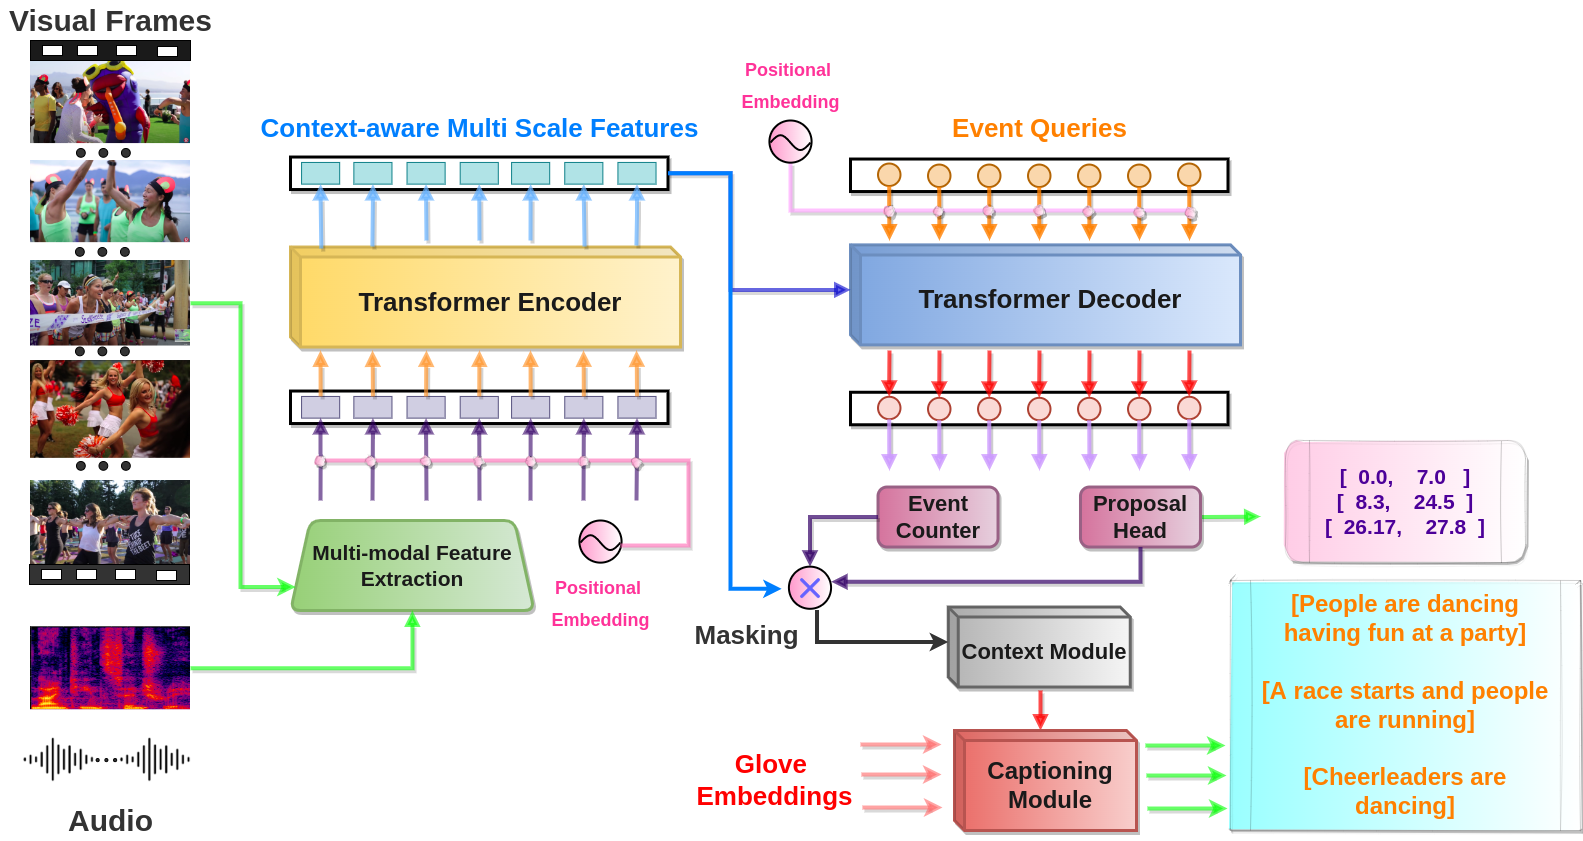
\includegraphics[width=\linewidth]{assets/img/architecture-no-bg.jpg}
	\caption{Proposed model architecture for Dense Video Captioning} %TODO add description?
\end{figure}

\section{Multimodal Feature Extraction}
\par Feature extraction is the backbone of our solution to tackle the task of Dense Video Captioning \cite{krishna2017densecaptioning}. A rich feature space would enhance the representational power of the model, thereby leading to more meaningful and accurate event proposals. Most previous works have utilized one modality only (i.e. video) to generate feature vectors as input to the proposal generator. However, audio cues, in conjunction with video frames is a strong event indicator. These events are accompanied with sharp changes in their corresponding audio spectrograms which can be learnt by the model to better determine the precise boundary of events. Thus, we aim to combine features generated using both video and audio. For this, we pre-train our encoders using the Temporally Sensitive Pre-training \cite{alwassel2021tsp} paradigm which is further explained in Chapter \ref{chapter:feat}.


\section{Proposal Generation}
\par Proposal generation is at the core of the dense video captioning task. It predicts the start and end time of events in the video which would then be used for captioning. Most previous works have used CNN-based architectures to predict event timestamps, but require a lot of fine-tuning to achieve competitive results.
\par We use an encoder-decoder architecture proposed by \cite{carion2020detr} and adapt it to work with videos across multiple modalities. Moreover, we implement deformable  attention \cite{zhu2020deformable} with token sparsification \cite{roh2021sparse} to decrease the quadratic time complexity of regular attention and improve event localization.
\par For all our losses, we assume $y$ as ground-truth events and $\hat{y}=\left \{ \hat{y_{i}} \right \}_{i=0}^{N}$ as the model predictions, where $N$ is the number of events in a batch.

\subsection{Transformer Encoder}
\par The transformer encoder consists of a deformable, multi-headed self-attention module followed by a feed-forward neural network (FFN). 
\par The encoder receives as input, multi-scale features $x_{0} \in R^{(N , d)}$ for $l$ feature levels, $N = \sum_{i=0}^{l-1}\left \{\frac{n}{i} \right \}$, where $d$ is the dimension of the model . The output of the encoder $m_{0} \in R^{(N , d)}$ belongs to a richer feature space tailored specifically for event localization and is treated as \textit{video memory} for the decoder. We also add fixed positional embeddings to each feature level of the input to overcome the permutation-invariance of transformers. 
\par We also use auxiliary loss (discussed in \ref{chapter:aux}) for all layers of the encoder except the last, which is used exclusively as input to the decoder.

\subsection{Transformer Decoder}
The transformer decoder consists of multi-headed self-attention and cross-attention modules (which can either follow the deformable or sparse attention paradigms) followed by a feed-forward neural network (FFN). The input to the decoder $q_{0} \in R^{(Q , d)}$ consists of $Q$ different embeddings, each representing a particular event in the video. Analogous to \cite{carion2020detr}, these $Q$ embeddings are learnt positional embeddings or \textit{event queries} and are added to the input (similar to the encoder). The decoder attends the \textit{event queries} with the \textit{video memory} and outputs embeddings $z_{0} \in R^{(Q , d)}$.
\par The output of the decoder is the fed to two prediction heads, namely the \textit{segment head} and the \textit{event counter}. The \textit{segment head} is a 3-layer FFN with the GELU activation function and and output dimension of 2, representing the normalized center-offset and length for an event. We calculate 2 losses for event segments, namely the $l1$ loss and the generalized $IoU$ (Intersection over Union) loss, normalized by the number of event segments in the batch.

$$\L_{l1} =  \left \| b_{i} - \hat{b_{i}} \right \| \hspace{1cm} \L_{giou} = \frac{\left |C\symbol{92}(A\cup B)   \right |}{\left | C \right |} $$

\par The \textit{event counter} consists of a single linear layer with an output dimension equaling the maximum predicted events in a video. Next, we use the $argmax$ function to find the $N_{set}$ followed by selecting the top-k events from the $N_{set}$ based on these confidence scores. We then calculate the cross-entropy loss $\L_{event}$ between the predicted, high-confidence event counts and the ground-truth event counts.

\subsection{Attention}
\par The attention mechanism proposed in \cite{tfm} has quadratic complexity as each token attends to every other token in the sequence. This may be important for text, but for images and videos (especially for the dense video captioning task), attending to a smaller set of tokens in a concentrated area is sufficient and can greatly reduce the time complexity. 
We implement deformable attention \cite{zhu2020deformable}, which attends to only a small set of key sampling points around a reference point, regardless of the spatial
size of the feature maps. Given an input feature map $x \in R^{C\times H \times W}$ , let q index a query element with content feature $z_q$ and a 2-d reference point $p_q$, the deformable attention feature is calculated by
$$ DeformAttn(z_q, p_q, x) = \displaystyle\sum\limits_{m=1}^M W_m
[\displaystyle\sum\limits_{k=1}^K A_{mqk}\cdot W'_mx(p_q+\Delta p_{mqk})]
$$
\par where k indexes the sampled keys, m indexes the attention head, and K is the total sampled key number. $\Delta p_{mqk}$ and $A_{mqk}$ denote the sampling offset and attention weight of the $k^{th}$ sampling point in the $m^{th}$ attention head, respectively.
\par Deformable attention module can be easily extended for multi-scale feature maps. Let $\{{x^l}\}_{l=1}^L$ be the input multi-scale feature maps, where  $x^l \in R^{C\times H^l \times W^l}$ . Let $ \hat p_q \in [0, 1]^2$ be the normalized coordinates of the reference point for each query element q, then the multi-scale deformable attention module is applied as

$$DeformAttn(z_q, \hat{p}_q, \{{x^l}\}_{l=1}^L) = 
\displaystyle\sum\limits_{m=1}^M W_m
[\displaystyle\sum\limits_{l=1}^L\displaystyle\sum\limits_{k=1}^K A_{mlqk}\cdot W'_mx^l(\phi _l (\hat p_q)+\Delta p_{mlqk})]$$

\par where l indexes the input feature level, m indexes the attention head, and k indexes the sampling point. $\Delta p_{mlqk}$ and $A_{mlqk}$ denote the sampling offset and attention weight of the $k^{th}$ sampling point in the $l^{th}$ feature level and the $m^{th}$ attention head, respectively

\par We further reduce the encoder tokens that should be further modified on the fly by
predicting a pseudo-ground truth of the saliency defined by decoder cross-attention maps \cite{roh2021sparse}.
The saliency of each input token is determined by aggregating the decoder cross-attentions between all \textit{event queries} and the encoder output. It generates a single map of the same size as the backbone’s feature map, which is known as the Decoder cross Attention Map (DAM). To train the scoring network, we binarize DAM so that only the top-k percentage of encoder tokens are
kept. To predict how likely a given encoder token is to be included in the top-p\% most referenced tokens, a 4-layer scoring network g is used, and the network is trained by minimizing the binary cross entropy (BCE) loss between the binarized DAM and prediction.

$$\L_{dam} = -\frac{1}{N}\displaystyle\sum\limits_{i=1}^N BCE(g(X_{feat})_i, DAM^{bin}_i)$$


\section{Context Mask Module}
\par Once the decoder predicts the events, we consider only those features of the video that belong to those particular events. For this, we use a differentiable masking network proposed by \cite{zhou2018end} instead of static masks used by most previous works.
\par The network is a simple FFN with an output dimension of $N=video\ sequence\ length$. It gets as input, normalized center offsets and lengths from the segment head and outputs a differentiable mask with values (near) zero when outside the event segments, and (near) one otherwise. Then, we perform an element-wise product with the \textit{video memory} produced by the encoder and feeds this output to the captioning module.
\par We use the Binary Cross-Entropy loss function between the binary (static) mask made using predicted event boundaries and the differentiable mask.

$$\L_{m} = \textrm{BCE}(\mathit{Bin}(S_{p}, E_{p}), f_{FFN}(S_{p}, E_{p}))$$


\begin{figure} [H]
	\centering
	\includegraphics[width=\linewidth]{assets/img/architecture-2.jpeg}
	\caption{Proposal Generation and Captioning using Context Masking Module} %TODO add description?
\end{figure}


\section{Captioning Module}
\par We use the transformer decoder proposed by \cite{tfm} along with 300-dimensional GloVe word embeddings pre-trained on 6 billion tokens\cite{glove}. The word embeddings are attended with the \textit{video memory} and output embeddings are fed into a softmax layer over the entire vocabulary to get next-word probabilities.
\par We use the KL divergence loss along with label smoothing to encourage small logit gaps and prevent the model from being too confident about its predictions.

$$y _{c}= (1 - \alpha)y_{onehot} + \frac{\alpha}{K} \hspace{1cm} \L_{cap}(y, \hat{y}) = \sum_{c=1}^{N}\hat{y} \log{\frac{\hat{y}}{y_c}}$$

\par where $K$ is the number of label classes, and $\alpha$ is a hyperparameter that determines the amount of smoothing.

\section{Event Set Prediction}
\par The output of the decoder consists of $Q$ event queries, each of which represents an event in the video with varying levels of confidence. $Q$ can be set based on the task complexities. Tasks such as object detection in images can have much more queries as compared to temporal action localization. The Hungarian matching algorithm \cite{hungarian} is used to suppress incorrectly assigned predicted segments to ground-truth instances when the decoder produces false positives or false negatives. We thus use a one-to-one mapping between the 2 sets and find only those assignments with the least cost (weighted bipartite matching).
\par We first calculating a cost matrix of each predicted segment against each ground truth segment. This cost is a linear combination of the $l1$ loss and the generalized $IoU$ loss.
$$ C = \alpha_{l1}\L_{l1}  + \alpha_{giou}\L_{giou}$$
\par Then, we use the Hungarian algorithm to optimally match predicted and ground truth segments by selecting the mappings with the lowest cost. Finally, we calculate the overall Hungarian loss across all selected segments for backpropagation through the entire model.

$$\L_{Hungarian}(y, \hat{y}) = \sum_{i=0}^{N}\left [ \alpha_{l1}\L_{l1} + \alpha_{giou}\L_{giou} + \alpha_{event}\L_{event} + \alpha_{m}\L_{m} + \alpha_{cap}\L_{cap} \right ]$$

\section{Auxiliary Losses} \label{chapter:aux}
\par To mitigate the problem of vanishing gradients and aid better learning throughput out the model, we utilize auxiliary losses during training for the transformer encoder, decoder and captioning module. We thus calculate the loss and backpropagate gradients for every layer of the model, just as we do for the final layer. However, we do not calculate the context mask loss as it is too expensive and requires more training time.
\par \cite{carion2020detr} does not calculate auxiliary loss for the encoder as its tokens are significantly more in number as compared to the decoder's tokens. However, due to sparsification from the decoder attention map, we can calculate the auxiliary loss for each layer in the encoder, but only for the selected tokens. 

\subsection{Gradient Flow}

\par Gradients and its flow is always a issue when dealing with large and complex models. With models based on the DETR \cite{carion2020detr} architecture, vanishing gradients is a problem. As suggested in \ref{chapter:aux}, we use auxiliary loss in the encoder as well. If we adopt the architecutre proposed in \cite{zhu2020deformable}, with no auxiliary loss for the encoder, the gradients through the encoder decrease at a rapid rate which in turn, reduces the rate at which the loss decreases. 
\par By using sparsification of encoder tokens and auxiliary loss across all layers of the encoder (except the last) as proposed in \cite{roh2021sparse}, the gradients do not vanish and are much more uniform across the entire model.

\begin{figure}[h]
	\centering
	\begin{subfigure}[b]{0.55\textwidth}
		\includegraphics[width=\linewidth]{assets/img/deformable_grad_flow_epoch_1.png}
	\end{subfigure}%
	\begin{subfigure}[b]{0.55\textwidth}
		\includegraphics[width=\linewidth]{assets/img/sparse_grad_flow_epoch_1.png}
	\end{subfigure}
	\caption{Gradient flow for epoch 1 (i). Deformable Transformer, (ii). Sparse Transformer}
	
	\label{fig:gradientflowepoch1}
\end{figure}

\begin{figure}[h]
	\centering
	\begin{subfigure}[b]{0.55\textwidth}
		\includegraphics[width=\linewidth]{assets/img/deformable_grad_flow_epoch_8.png}
	\end{subfigure}%
	\begin{subfigure}[b]{0.55\textwidth}
		\includegraphics[width=\linewidth]{assets/img/sparse_grad_flow_epoch_8.png}
	\end{subfigure}
	\caption{Gradient flow for epoch 8 (i). Deformable Transformer, (ii). Sparse Transformer}
	
	\label{fig:gradientflowepoch8}
\end{figure}







% section
\section{Feature Extraction}
\par For the task of Dense Video Captioning, a rich feature space would enhance the representational power of the model, thereby leading to more meaningful and accurate event proposals and captions. In most previous works, convolutional neural networks are commonly used to extract features  from videos for any downstream tasks. Moreover, most localization methods use video features extracted by models that are trained for the task of Trimmed Action Classification (TAC), on datasets such as Kinetics\cite{kay2017kinetics} and Sports-1M, such as R(2+1)D\cite{r(2+1)d}, I3D\cite{carreira2018quo}, C3D and others. Additionally, most previous works focus on using a single modality (i.e. video) or multiple modalities based only on video, like RGB and optical flow features, for example from I3D\cite{carreira2018quo}, to generate feature vectors as input to the downstream model. Some works have used multiple modalities including video (RGB, optical flow) and audio, like \cite{iashin2020better}. The motivation for using multiple modalities is so that the feature space can grow richer, and that multiple modalities can complement each other to give strong event indicators. 

\par In this section, we explain how features are extracted from videos in the form of two modalities: video and audio. We use the \textit{Video Vision Transformer (ViViT)} \cite{vivit} for video feature extraction and the \textit{Audio Spectogram Transformer (AST)} \cite{ast} for audio feature extraction. We also consider the temporal sensitivity of features as a characteristic that can benefit DVC.

\subsection{Feature Extraction Methodology}


\subsubsection{Video Features Extraction Using ViViT} \label{video-feat-extraction}
\par Video features are the most important part of the encoder. Without a robust and rich feature space for videos, the downstream model would never be able to learn accurate event boundaries or captions. Previous state-of-the-art video encoders \cite{carreira2018quo}, \cite{csn}, \cite{r(2+1)d} use CNN-based architectures. Although they have strong inductive bias and translation invariance, they fail to model long-range temporal dependencies which are of importance when encoding videos. Moreover, CNNs require different architectures to model different modalities which can become complex when combining multiple modalities such as video and audio. Transformers \cite{tfm} can overcome these barriers using their attention mechanism without compromising on statistical and computational efficiency. Moreover, transformers can use the same building blocks across different modalities without many modifications. We aim to use the recently proposed ViViT model \cite{vivit}, a purely attention-based video encoder which has outperformed previous approaches for action recognition such as  Kinetics 400 and 600, Epic
Kitchens 100, Something-Something v2 and Moments in Time. Even though ViViT requires several orders of magnitude more training data as compared to its CNN counterparts, the authors of ViViT propose several methods to limit its training requirements by using pretrained weights in conjunction with strong regularization and specific fine-tuning.

\begin{figure} [H]
	\centering
	\includegraphics[width=7cm, height=6cm] {assets/img/vivit_methodology.png}
	\caption{ViViT encoder by Dosovitskiy \textit{et al}. (Image courtesy \cite{vivit})}
\end{figure}

% TODO: Working of VIVIT, video frames augmentation and preprocessing

\par Arnab \textit{et al} propose two methods for mapping a video to its corresponding embeddings for input to ViViT, \textit{Uniform frame sampling} and \textit{Tubelet embedding} in \cite{vivit}. We use the uniform frame sampling method in our feature extraction framework. Arnab \textit{et al} also propose different attention mechanisms for the ViViT model; we use the \textit{spatio-temporal attention} mechanism. The flow of data is as follows:

\begin{enumerate}
	\item Consider the original video clip $X$ as consisting of $T$ frames, each of width $W$ and height $H$. The video has $C$ channels. Hence the shape of video frames of $X$ is $(T, H, W, C)$.
	\item We perform certain preprocessing steps on the video frames:
	\begin{enumerate}
		\item We resize the spatial dimensions of the video frames. The shorter edge is resized to $256$, and the longer edge is resized maintaining the aspect ratio.
		\item We normalize all channels of the video frames.
		\item Generalizability and robustness of the features motivate data augmentation of the video frames. To this end, we randomly flip the video frames horizontally, and take random crops of spatial dimensions $224 \times 224 $ during training. Note that for validation and inference, we skip the random horizontal flip step and take a center crop of the same dimensions.
	\end{enumerate}
	\item Now, the uniform frame sampling method proposed by Arnab \textit{et al} in 
\cite{vivit} is used to extract tokens mapped to a $768$-dimensional space. This involves using a three-dimensional convolutional layer to project the frames to patch embeddings, so that the shape of the embeddings are $(T, N, 768)$, where $N$ is the number of patches.
	\item The patch embeddings are then flattened to $(T \times N, 768)$, and concatenated with a \textit{class token} for input to the encoder layers of ViViT.
	\item For each encoder layer, the input is subject to (1) positional encoding, (2) layer normalization, (3) multi-head self-attention across all tokens, (4) layer normalization and (5) two fully connected layers with GeLU activation and dropout.
	\item Finally, the class token from the output of the last encoder layer is used as the feature representation of the clip $X$.
\end{enumerate}

\par More details about the different frame sampling methods, attention mechanisms and the ViViT model are given in \ref{appendix:vivit-paper}

\subsubsection{Audio Features Extraction using AST} \label{audio-feats-extraction}
\par Audio is an important aspect of any video. Not only does audio suggest the duration of an event, it can also signify the magnitude or significance of that event. Thus, audio becomes a powerful accessory to images when representing a video. We aim to use the recently proposed Audio Spectogram Transformer (AST) \cite{ast} which has outperformed current state-of-the-art models in audio classification.
\begin{figure} [H]
	\centering
	\includegraphics[width=7cm, height=6cm] {assets/img/ast_methodology.png}
	\caption{AST encoder by Gong \textit{et al}. (Image courtesy \cite{ast})}
\end{figure}

% TODO: Working of AST, Mel Spectograms and audio preprocessing

\subsection{Temporal Sensitivity of Features}
\par As mentioned previously, most localization methods use video features extracted by models that are trained for Trimmed Action Classification (TAC) tasks. These features are not necessarily optimal for Temporal Action Localization (TAL) and other dependent tasks such as Action Proposal Generation and Dense Video Captioning. Alwassel \textit{et al}, in their paper titled \textit{TSP: Temporally Sensitive Pretraining of Video Encoders for Localization Tasks}, claim that this is due to the inherent lack of temporal sensitivity in features from TAC trained video encoders \cite{alwassel2021tsp}. Yet, these features are prominently used for TAL and DVC tasks. This discrepancy is explained by the following reasons:
\begin{itemize}
	\item Due to a lot of existing research for TAC tasks, a lot of established models exist that can be used off the shelf for video feature extraction
	\item The video encoders usually cannot be directly trained along with downstream tasks of TAL or DVC due to resource constraints; it is impractical to fit long untrimmed videos in commodity GPUs without drastically downsampling them in terms of space or time.
\end{itemize}

\par To solve this problem, Alwassel \textit{et al} introduced a supervised pre-training paradigm for TAL that aims to instill the ability to produce temporally sensitive features; video encoders are trained to explicitly discriminate between foreground and background clips in untrimmed videos. They show that TSP improves performance for TAL, action proposal and DVC tasks consistently on different datasets as well as with different downstream predictive models and architectures, clearly establishing that temporally sensitive features contribute positively to the task at hand. TSP involves training encoders with a downstream task involving two classification heads: (1) \textit{action classification} head and (2) \textit{temporal region classification} head. This architecture is applied to clips from untrimmed videos. Optionally, along with local features of every clip, a \textit{global video feature (GVF)} is also used for the temporal region classification to further improve temporal sensitivity \cite{alwassel2021tsp}. A summary of their work is given in \ref{appendix:tsp-paper}.


\subsubsection{Temporally Sensitive Pretraining of Proposed Feature Extractors}

\par We extend the TSP framework proposed by Alwassel \textit{et al} \cite{alwassel2021tsp} to use temporally sensitive features in our work for DVC.

\paragraph{Architecture} The model used for TSP consists of one or more \textit{backbone} architectures for particular modalities, which in our case are ViViT - for video modality, and AST - for audio modality. The constructed model is such that different backbones and their modalities can be plugged in and out as required for experimentation. The input modality data of a clip is fed in to each backbone separately, and the output feature representations from each backbone are combined and passed through a fully connected layer to give a final feature representation. This feature representation is fed into the action classification head and the temporal region classification head to give the respective outputs. Note that we do not use a GVF in the current implementation of our pretraining framework, and plan to include this in later work.

\begin{figure}
\centering
\includegraphics[width=\linewidth]{assets/img/tsp/tsp-arch.png}
\caption{The proposed feature extraction framework with ViViT and AST backbones. TSP heads for action classification and temporal region classification are shown on the right.}
\label{fig:tsp-arch}
\end{figure}

\paragraph{Data Flow} In our case, the following data flow is followed (considering two backbones: ViViT and AST):
\begin{enumerate}
	\item Video frames are extracted from the clips, and are preprocessed and augmented as mentioned in \ref{video-feat-extraction} making the features at this level of the shape $(B, C, T, H, W)$, where $B$ is the batch size, $C$ is the number of channels (3 for RGB), $T$ is the temporal length of the clip in terms of number of frames and $H$ and $W$ are the height and width (spacial dimensions) of each frame in the clip respectively.
	\item Audio frames are extracted from the clips as explained in \ref{audio-feats-extraction}. At this stage, they are of the shape $(B, N, F)$, where $N$ is the number of time frames and $F$ is the frequency bins.
%TODO Check AST dims and meanings
	\item Video features of the shape $(B, C, T, H, W)$ are fed into ViViT, and the class token of shape $(d_v, )$ of ViViT is used as the feature representation $f_v$ of the video modality of the clip.
	\item Audio features of the shape $(B, N, F)$ are fed into AST, and the class token of the shape $(d_a, )$ of AST is used as the feature representation $f_a$ of the audio modality of the clip.
	\item These two features, $f_a$ and $f_v$, are then combined using some function, for example addition or concatenation. In general, if there are $n$ backbones and we have features $f_1, f_2, f_3, ..., f_n$, this combiner function must combine all these and give a single-dimensional feature $f'$ of dimensions $(d', )$. 
	\item The feature $f'$ is fed into a fully connected layer that converts it into a feature $f$ of shape $(d, )$. This feature $f$ is the final feature representation that is used for downstream tasks.
	\item $f$ is fed to the action classification head, which consists of a simple fully connected layer followed by softmax activation layer, to give the action classification logits $y_c$ as output.
	\item $f$ is also fed (optionally combined with the GVF, $f_g$, to improve the temporal sensitivity of the feature representation) to the temporal region classification head, which consists of a fully connected layer followed by the sigmoid activation layer, to give the binary temporal region classification logit $y_r$ as output.
\end{enumerate}
\par The global video feature is extracted in the same manner as local features, with the additional step of \textit{pooling} across all local features ${f_1, f_2, ..., f_n}$ for a video. 

\paragraph{Loss functions} As mentioned, there are two classification heads on the top of the TSP framework:
\begin{itemize}
	\item \textbf{Action Classification}: This head predicts action classes for a given input clip. The head can be represented as $f \rightarrow y_c$. The cross-entropy loss function is used for this head, with mean reduction ($L_c$):
$$ L_{CE} = -\frac{1}{n} \sum_{i=1}^{n}{\textbf{y}log(\hat{\textbf{y}})} $$
	\item \textbf{Temporal Region Classification}: This head predicts temporal region classes for a given input clip, i.e. whether the particular clip lies in an action (foreground) temporal region or non-action (background) temporal region. The head can be represented as $f \rightarrow y_r$. For binary classification, the cross entropy function reduces to binary cross entropy ($L_r$).
\end{itemize}
\par The two losses, $L_c$ and $L_r$ are given loss coefficients $\alpha_c$ and $\alpha_r$ for relative importance for contributing towards the total loss:
$$ L = \alpha_c L_c + \alpha_r L_r $$

\par We evaluate the effectiveness of this temporally sensitive pretraining in the Results section.
%TODO Make results a ref, and add TSP eval



\chapter{Experimentation and Results}
\section{Experimentation}
\par We implement the feature extraction framework and the model architectures in PyTorch. We show that our model achieves competitive results compared to current state-of-the-art models with fewer training epochs and even fewer attention tokens. We utilize multimodal features from ViViT and AST encoders, pretrained using our adapted Temporally Sensitive Pretraining framework. The ActivityNet dataset is used, which is the largest available dataset for the task of Dense Video Captioning.

\subsection{Feature Preprocessing Details}
\par We standardize all videos in the ActivityNet Captions dataset to 30 frames per second (30fps) and audio sampling rate of 44100Hz. For feature extraction as well as temporally sensitive pretraining, we use 16 frames per clip and sample 5 clips per segment in the dataset. We use 128 Mel bins and a target length of 64 for audio input. We start training the ViViT and AST encoders from Kinetics pretrained weights and Audioset pretrained weights respectively. ViViT uses a spatial patch size of $16 \times 16$, and a temporal patch size of 2. The number of encoder layers of ViViT and AST is kept 12. We train these encoders with a batch size of 8 and a stochastic gradient descent optimizer with momentum and weight decay.

\subsection {Training Details}
\par We train our model across 4 DGX-A100 GPUs for 70 epochs with an NCCL backend and a batch size of 16 for 60 hours. We use the AdamW optimizer with a learning rate of $10^{-4}$. We also use gradient clipping with a maximum threshold of $0.1$ to avoid exploding gradients. We set the model's embedding dimension to 512, with 6 layers and 8 attention heads for the transformer encoder, decoder and captioning module. Thus, our model has 75M parameters, excluding the feature extraction encoders. 
\par The smoothing rate $\alpha$ (for caption loss) is set to $0.5$. We initialize all transformer weights using the Xavier initialized distribution \cite{xavier}. We also use $sine$ positional embeddings, adapted for videos by accounting for their duration. We set the number of \textit{event queries} to 20 and the maximum event counter length to 10.
\par For the deformable attention head, we use 4 feature levels with 4 sampling sampling points per attention head and a 2048-dimensional FFN. We set $\rho$ to 0.5 (utilize only 50\% tokens) and dropout as 0.1.
\par For calculating the Hungarian loss, we perform a linear combination across all individual losses. Their corresponding coefficients are $\alpha_{l1}=5, \alpha_{giou}=2, \alpha_{event}=2, \alpha_m=3, \alpha_{cap}=1$.

\subsection {Evaluation Metrics}
\par We use 2 different metric sets to evaluate different aspects of our model.
\begin{itemize}
	\item For evaluating the event boundaries, we use Precision and Recall across IoU thresholds at $\left \{0.3, 0.5, 0.7, 0.9 \right\}$ along with an average across all the thresholds. We also calculate the corresponding average F1 score.
	\item For evaluating the captions, we calculate the BLEU \cite{bleu} scores across 4 thresholds at $\left \{1, 2, 3, 4\right\}$, METEOR \cite{meteor} and CIDEr \cite{cider}, based on the official ActivityNet challenge guidelines. We also calculate the ROUGE-L \cite{rouge} scores for the captions.
\end{itemize}

\section{Results}

Our model achieves competitive results for both, the event localization and event captioning tasks across most metrics. The following tables show the results of the comparison for captioning and event localization against popular previous works, each with different model architectures and training paradigms.
% Please add the following required packages to your document preamble:
% \usepackage{multirow}
\begin{table}[h] \label{table:capeval}
	\centering
	\begin{tabular}{|c|cclllcc|}
		\hline
		\multirow{2}{*}{\textbf{Paper}}        & \multicolumn{7}{c|}{\textbf{Learnt Proposals}}                                                                                                                                                                                                                        \\ \cline{2-8} 
		& \multicolumn{1}{c|}{M}             & \multicolumn{1}{c|}{C}              & \multicolumn{1}{c|}{R}               & \multicolumn{1}{l|}{B@1}             & \multicolumn{1}{l|}{B@2}           & \multicolumn{1}{c|}{B@3}           & B@4                                \\ \hline
		{Krishna \textit{et al} \cite{krishna2017densecaptioning} DCE}                                 & \multicolumn{1}{c|}{5.69}          & \multicolumn{1}{c|}{12.43}          & \multicolumn{1}{l|}{}                & \multicolumn{1}{l|}{10.81}           & \multicolumn{1}{l|}{4.57}          & \multicolumn{1}{c|}{1.90}          & 0.71                               \\ \hline
		{Zhou \textit{et al} \cite{zhou2018end} Masked Transformer}                & \multicolumn{1}{c|}{4.98}          & \multicolumn{1}{c|}{9.25}           & \multicolumn{1}{l|}{}                & \multicolumn{1}{l|}{9.96}            & \multicolumn{1}{l|}{4.81}          & \multicolumn{1}{c|}{2.42}          & 1.15                               \\ \hline
		{Wang \textit{et al} \cite{wang2018bidirectional} Bi-SST}                       & \multicolumn{1}{c|}{5.86}          & \multicolumn{1}{c|}{7.99}           & \multicolumn{1}{l|}{\textbf{19.29}}           & \multicolumn{1}{l|}{\textbf{19.37}}           & \multicolumn{1}{l|}{\textbf{8.84}}          & \multicolumn{1}{c|}{2.55}          & 1.31                               \\ \hline
		{Li \textit{et al} \cite{li2018jointly} Descriptivness Regr.}          & \multicolumn{1}{c|}{6.93}          & \multicolumn{1}{c|}{13.21}          & \multicolumn{1}{l|}{}                & \multicolumn{1}{l|}{12.22}           & \multicolumn{1}{l|}{5.72}          & \multicolumn{1}{c|}{2.27}          & 0.74                               \\ \hline
		{Mun \textit{et al} \cite{mun2019streamlined} Streamlined DVC}               & \multicolumn{1}{c|}{8.82}          & \multicolumn{1}{c|}{30.68}          & \multicolumn{1}{l|}{}                & \multicolumn{1}{l|}{17.92}           & \multicolumn{1}{l|}{7.99}          & \multicolumn{1}{c|}{2.94}          & 0.93                               \\ \hline
		Rahman \textit{et al} \cite{rahman2019watch} Watch, Listen, Tell       & \multicolumn{1}{c|}{4.93}          & \multicolumn{1}{c|}{13.79}          & \multicolumn{1}{l|}{10.39}           & \multicolumn{1}{l|}{10}              & \multicolumn{1}{l|}{4.2}           & \multicolumn{1}{c|}{1.85}          & 0.9                                \\ \hline
		Suin \textit{et al} \cite{suin2020efficient} Efficient framework for DVC & \multicolumn{1}{c|}{6.21}          & \multicolumn{1}{c|}{13.82}          & \multicolumn{1}{l|}{}                & \multicolumn{1}{l|}{}                & \multicolumn{1}{l|}{}              & \multicolumn{1}{c|}{2.87}          & 1.35                               \\ \hline
		Iashin \textit{et al} \cite{iashin2020multimodal} Multi-modal DVC            & \multicolumn{1}{c|}{7.31}          & \multicolumn{1}{l|}{}               & \multicolumn{1}{l|}{}                & \multicolumn{1}{l|}{}                & \multicolumn{1}{l|}{}              & \multicolumn{1}{c|}{2.6}           & 1.07                               \\ \hline
		Iashin \textit{et al} \cite{iashin2020better} BMT                       & \multicolumn{1}{c|}{8.44}          & \multicolumn{1}{l|}{}               & \multicolumn{1}{l|}{}                & \multicolumn{1}{l|}{}                & \multicolumn{1}{l|}{}              & \multicolumn{1}{c|}{\textbf{3.84}}          & 1.88                               \\ \hline
		Xiong \textit{et al} \cite{xiong2018forward} Move Forward and Tell      & \multicolumn{1}{c|}{7.08}          & \multicolumn{1}{l|}{}               & \multicolumn{1}{l|}{}                & \multicolumn{1}{l|}{}                & \multicolumn{1}{l|}{}              & \multicolumn{1}{c|}{2.84}          & 1.24                               \\ \hline
		{Wang \textit{et al} \cite{wang2020densecaptioning} SYSU}                        & \multicolumn{1}{c|}{\textbf{10.31}}         & \multicolumn{1}{l|}{}               & \multicolumn{1}{l|}{}                & \multicolumn{1}{l|}{}                & \multicolumn{1}{l|}{}              & \multicolumn{1}{c|}{}              &                                    \\ \hline
		Chadha \textit{et al} \cite{chadha2020iperceive} iPerceive                 & \multicolumn{1}{c|}{7.87}          & \multicolumn{1}{l|}{}               & \multicolumn{1}{l|}{}                & \multicolumn{1}{l|}{}                & \multicolumn{1}{l|}{}              & \multicolumn{1}{c|}{2.93}          & 1.29                               \\ \hline
		Song \textit{et al} \cite{songruc} RUC Sequential Events                 & \multicolumn{1}{c|}{8.82}          & \multicolumn{1}{l|}{30.68}               & \multicolumn{1}{l|}{}                & \multicolumn{1}{l|}{17.92}                & \multicolumn{1}{l|}{7.99}              & \multicolumn{1}{c|}{2.94}          & 0.93                               \\ \hline
		Deng \textit{et al} \cite{deng2021sketch} Sketch, Ground and Refine   & \multicolumn{1}{c|}{9.37}          & \multicolumn{1}{c|}{22.12}          & \multicolumn{1}{l|}{}                & \multicolumn{1}{l|}{14.05}           & \multicolumn{1}{l|}{}              & \multicolumn{1}{c|}{}              & 1.67                               \\ \hline
		Chen \textit{et al} \cite{chen2021towards} Towards Bridging EC-SL      & \multicolumn{1}{c|}{7.49}          & \multicolumn{1}{c|}{21.21}          & \multicolumn{1}{l|}{13.02}           & \multicolumn{1}{l|}{13.36}           & \multicolumn{1}{l|}{5.96}          & \multicolumn{1}{c|}{2.78}          & 1.33                               \\ \hline
		{Alwassel \textit{et al} \cite{alwassel2021tsp} TSP with BMT}            & \multicolumn{1}{c|}{8.75}          & \multicolumn{1}{l|}{}               & \multicolumn{1}{l|}{}                & \multicolumn{1}{l|}{}                & \multicolumn{1}{l|}{}              & \multicolumn{1}{c|}{4.16}          & \textbf{2.02}                               \\ \hline
		Wang \textit{et al} \cite{wang2021endtoend} Parallel decoding           & \multicolumn{1}{c|}{8.08}          & \multicolumn{1}{c|}{28.59}          & \multicolumn{1}{l|}{}                & \multicolumn{1}{l|}{}                & \multicolumn{1}{l|}{}              & \multicolumn{1}{c|}{}              & 1.96                               \\ \hline
		\textbf{Our model (video only)}                     & \multicolumn{1}{c|}{\textbf{6.42}} & \multicolumn{1}{l|}{\textbf{30.22}} & \multicolumn{1}{l|}{\textbf{13.58}} & \multicolumn{1}{l|}{\textbf{13.44}} & \multicolumn{1}{l|}{\textbf{4.12}} & \multicolumn{1}{l|}{\textbf{1.88}} & \multicolumn{1}{l|}{\textbf{0.44}} \\ \hline
		\textbf{Our model (video \& audio)}                     & \multicolumn{1}{c|}{\textbf{6.61}} & \multicolumn{1}{l|}{\textbf{31.38}} & \multicolumn{1}{l|}{\textbf{14.46}} & \multicolumn{1}{l|}{\textbf{15.36}} & \multicolumn{1}{l|}{\textbf{6.09}} & \multicolumn{1}{l|}{\textbf{2.28}} & \multicolumn{1}{l|}{\textbf{0.80}} \\ \hline
	\end{tabular}
	
	\centering
	\caption{Performance comparison of previous methods on the ActivityNet Captions dataset (*some videos unavailable)}  \label{tab: performance-comparison}
	
\end{table}

% Please add the following required packages to your document preamble:
% \usepackage{multirow}
\begin{table}[]
	\centering
	\begin{tabular}{|c|ccc|}
		\hline
		\multirow{2}{*}{\textbf{Paper}} & \multicolumn{3}{c|}{\textbf{Learnt Proposals}}                                             \\ \cline{2-4} 
		& \multicolumn{1}{c|}{Precision}      & \multicolumn{1}{c|}{Recall}         & F1             \\ \hline
		Zhou \textit{et al} \cite{zhou2017automatic} ProcNets                   & \multicolumn{1}{c|}{30.4}           & \multicolumn{1}{c|}{37.1}           & 33.42          \\ \hline
		Iashin \textit{et al} \cite{iashin2020better} BMT                             & \multicolumn{1}{c|}{48.23}          & \multicolumn{1}{c|}{\textbf{80.31}}          & 60.27          \\ \hline
		{Wang \textit{et al} \cite{wang2018bidirectional} Bi-SST}             & \multicolumn{1}{c|}{44.8}           & \multicolumn{1}{c|}{57.6}           & 50.40          \\ \hline
		Wang \textit{et al} \cite{wang2021endtoend} Parallel decoding                            & \multicolumn{1}{c|}{58.07}          & \multicolumn{1}{c|}{55.42}          & 56.71          \\ \hline
		{Mun \textit{et al} \cite{mun2019streamlined} Streamlined DVC}                 & \multicolumn{1}{c|}{57.57}          & \multicolumn{1}{c|}{55.58}          & 56.56          \\ \hline
		Song \textit{et al} \cite{songruc} RUC Sequential Events           & \multicolumn{1}{c|}{58.65}          & \multicolumn{1}{c|}{55.79}          & 57.18          \\ \hline
		\textbf{Our model (video)}              & \multicolumn{1}{c|}{\textbf{62.14}} & \multicolumn{1}{c|}{\textbf{61.25}} & \textbf{61.69} \\ \hline
		\textbf{Our model (video \& audio)}              & \multicolumn{1}{c|}{\textbf{66.25}} & \multicolumn{1}{c|}{\textbf{65.92}} & \textbf{66.08} \\ \hline
	\end{tabular}

	\centering
	\caption{Precision-Recall comparison of previous methods on the ActivityNet Captions dataset (*Some videos unavailable)}  \label{tab: precision-recall-comparison}
\end{table}




\chapter{Conclusion and Future Work}
\section{Conclusion}

\par Dense Video Captioning is an extremely complex task that is can be considered as the culmination of various tasks in the field of Computer Vision as well as Natural Language Generation. It has numerous applications in different areas in the upcoming digital age, and so developing a solution for this problem is well motivated.

\par A performant DVC model requires multiple sequential modules, each with millions of parameters and numerous losses. We proposed a novel solution that improves upon the shortcomings of previous works by introducing multiple modalities, employing efficient attention mechanisms and using contextual learning to aid the end-to-end training paradigm. Multiple modalities lead to richer feature spaces compared to single modality features, while an end-to-end training paradigm promotes inter-task promotion for the proposal generation and captioning tasks. The use of attention mechanisms and transformer architectures for the task of DVC is relatively unexplored, hence we investigate the effectiveness of these for DVC.

\par First, we propose a feature extraction framework to generate temporally sensitive multimodal features using the Video Vision Transformer and Audio Spectrogram Transformer, providing a rich representation space for the model to work with. Along the way, we also evaluate the effectiveness of temporally sensitive features qualitatively and quantitatively.

\par Next, we propose a novel transformer-based architecture consisting of a encoder-decoder proposal generation module, a contextual learning module and a decoder-based captioning module. Each of these modules work in tandem to first encode the pre-trained multimodal features, followed by predicting the timestamps of all the events in the video along with a count of the number of events in the video. These parameters are then used to build a differentiable context mask which masks those tokens of the video that are not in the specific event under consideration. This aids in end-to-end training and backpropagates losses across the decoder as well (which would not have been possible if we used a static mask). Finally, the localized event features are fed into the caption decoder to predict next-work probabilites over the entire vocabulary.

\par We achieve competitive results against previous works over a range of evaluation metrics and provide detailed analysis and our qualitative interpretation on them. We also evaluate how well the model learns across a variety of settings and select the best one.

\par The challenges we faced during this project mainly stemmed from the huge sizes of video and audio data as well as the large models necessary for processing this data and predicting reasonable proposals and captions. These include high training time, memory constraints, and consequent problems in iterative improvement of our model. 	

\section{Future Work}
\par Dense Video Captioning is a complex task which requires hours of training and hyper-parameter tuning to get optimized results for both, the event localization and caption generation. In the future, we would build on top of our current results by: 
\begin{itemize}
	\item Using 768-dimensional feature vectors throughout our model. This would double the parameters in our model from 75M to 150M and thereby, would require longer training schedules on multiple GPUs.
	\item Training the model on other datasets such as YouCook, YouCook2, TACoS, Kinetics, etc. for tasks, dense video captioning, classification and localization.
	\item Separating the input modalities throughout the model with cross attention between the two. This however, would significantly increase the model size and we would then be able to run it on high compute GPUs only. 
	\item Thus, we would also try further optimizations such as to make the model suitable to run on low compute platforms.
	\item We would also work on adapting the model to various other tasks such as VQA (Visual Question Answering), video summarization and video retrieval.
\end{itemize} 




\appendix
\settocdepth{section}


% \chapter{Supplementary Details}
% Include individual suppl-detail file here
% Use section as the top level section in that .tex file


\chapter{Paper Summaries}
% Include individual paper summaries here
% Use section as the top level section in that .tex file
\subsection{Dense-Captioning Events in Videos}

\subsubsection{Overview}

\par Ranjay Krishna \textit{et al}, in their 2017 paper titled \textit{Dense-Captioning Events in Videos} \cite{krishna2017densecaptioning}, proposed the problem of \textit{dense video captioning}. The network was able to output overlapping events and events with varying time scales. The captioning module output also considered past and future context of the representative event. They also introduced new datset with over 20K annotated videos for this problem - ActivityNet Captions.


\subsubsection{Datasets}
\begin{itemize}
\item ActivityNet Captions
\end{itemize}

\subsubsection{Performance}
\par Krishna \textit{et al} compared captioning results with LSTM-YT\cite{venugopalan2015sequence}, S2VT\cite{venugopalan2015translating} and H-RNN\cite{yu2016video} using BLEU@1-4, METEOR and CIDEr. Since these models were only for captioning, the results were compared by providing ground-truth proposal boundaries. The metrics showed better results even when their pipeline generated captions on learnt proposals. The model was tested with different type of contexts input in captioning model, and full-context (\textit{both past and future}) proved to better for longer videos. The results of event localization depicted how multi-stride network performed better for videos with more number of events. The model also reported state-of-the-art results for the task of vdeo and paragraph retrieval


\subsubsection{Methodology}

\par Krishna \textit{et al} architecture consists of two main components:
\begin{enumerate}
	\item Event proposal module
	\item Captioning module with context
\end{enumerate}

\begin{figure}[h]
	\includegraphics[width=\linewidth]{assets/img/krishna2017densecaptioning-architecture.png}
	\caption{Pipeline introduced by Krishna \textit{et al} (Image courtesy \cite{krishna2017densecaptioning})}
\end{figure}

\paragraph{Flow of pipeline}
\begin{enumerate}
	\item C3D features of sampled video frames.
	\item Sampling done at different strides to capture all kind of events.
	\item Features fed into LSTM type of network inspired by DAPs\cite{Escorcia2016DAPsDA} for generating proposals.
	\item Captioning module used a LSTM network with following inputs:
	\begin{enumerate}
		\item hidden representation of past events $h_i^{past}$
		\item hidden representation of current event $h_i$
		\item hidden representation of future events $h_i^{future}$
	\end{enumerate}
\end{enumerate}


\subsubsection{Conclusion}

\par Krishna \textit{et al} tackled the task of captioning videos with correlation between events. They also showed the results on streaming videos with current event relating to only past events.
\newpage
\section{A Better Use of Audio-Visual Cues: Dense Video Captioning with Bi-modal Transformer}

\subsection{Overview}

\par Iashin and Rahtu, in their 2020 paper titled \textit{A Better Use of Audio-Visual Cues} \cite{iashin2020better},
approached the task of Dense Video captioning by using two types of input features: video as well as
audio. They identified the lack of research into utilizing the audio track of videos to generate
dense captions, despite the natural co-occurence of the two. They introduce a nove \textit{Bimodal
Transformer} which has the similar encoder-decoder architecture as the traditional Transformer model, 
but generalizes it to two input modalities:  audio features (using VGGish \cite{vggish}) and visual 
features (using I3D \cite{carreira2018quo}). Their  framework also consists of a \textit{multiheaded bimodal 
proposal generator}, inspired by the \textit{YOLO} object detector \cite{yolo} which generates event 
proposals for caption generation.


\subsection{Datasets}
\begin{itemize}
\item ActivityNet Captions \cite{krishna2017densecaptioning}
\end{itemize}

\subsection{Performance}
\par Iashin \textit{et al} report state-of-the-art-performance for the dense video captioning 
task on the published validation subset of the ActivityNet Captions dataset in terms of BLEU@3-4 
metrics and near state-of-the-art performance in terms of the METEOR metric. Considering the 
task of proposal generation in isolation, they report state-of-the-art performance with the F1 
score of 60.27\%, on the same dataset.


\subsection{Methodology}

\par Iashin \textit{et al} use a Inflated 3D Network pre-trained on the \textit{Kinetics} dataset
\cite{kay2017kinetics} for extracting visual features from video
frames. For audio features, the VGGish network \cite{vggish} is used. These features are stacked in 
sequence for each video. The caption tokens are embedded with pre-trained \textit{GloVe} \cite{glove}.

\begin{figure}[h]
	\includegraphics[width=\linewidth]{assets/img/bmt-architecture.png}
	\caption{Dense Video Captioning Framework introduced by Iashin \textit{et al} (Image courtesy \cite{iashin2020better})}
\end{figure}


\par The design proposed by Iashin \textit{et al} consists of two major functional components:
\begin{itemize}
\item Bi-modal Transformer
\item Multiheaded Proposal Generator
\end{itemize}

For inference, the features flow through the components as follows:
\begin{enumerate}
\item Both feature sequences, audio $A$ and visual $V$ are self-attended and then passed
through an $N$-layered encoder to produce bi-modal sequence representations using novel
bi-modal multi-headed attention blocks to fuse features from both sequences. These bimodal
attention blocks output two sequences of features, $A^v$ (visual attended audio features)
and $V^a$ (audio attended visual features).

\item $A^v$ and $V^a$ are then given to the Proposal Generator, which consists of two
distinct sets of \textit{proposal generator heads}, one set for each input modality.
Each proposal generator head makes proposal predictions at each time step independently,
forming a common pool of cross-modal predictions. Top $k$ predictions are selected (using a
confidence score) from this pool to be the output of the proposal generator: the proposals.

\item The generated proposals are used to clip the input feature sequences which are then
given to the Bimodal Encoder. The same self-attention followed by bimodal attention is
carried out on these clipped features.

\item The encoder's outputs are passed to the bi-modal attention blocks in every decoder
layer of the Bimodal Decoder, along with the representation of previously generated caption
words. The caption embeddings are self-attended, and then carries out bi-modal
encoder-decoder attention, producing $C_n^{A^v}$ (audio-visual attended previous captions)
and $C_n^{V^a}$ (visual-audio attended previous captions). After a bridge connection and
positional encoding (to add order information to the permutation invariant transformer
architecture), two fully connected layers with ReLU activation between them and a softmax
activation in the final layer are used to model the distribution of the next caption token 
over the vocabulary.

\end{enumerate}

\subsubsection{Proposal Generation Module}


\par The design of individual proposal generator heads in the Proposal Generator is inspired by 
the YOLO object detector \cite{yolo}. A set of anchors is determined apriori by running 
K-Means Clustering on the ground truth event lengths. Each centroid of the cluster is taken 
as an anchor in the anchor set $\psi$. The distance metric used here is the Euclidean 
distance, in contrast to IoU (Intersection over Union) used in YOLO. Each proposal generator 
head predicts three values: (1) center of the event $c$, (2) log coefficient $l$ and (3) 
objectness score $o$. Using these values, the temporal boundaries and confidence of the event 
predicted are calculated:

$$ center = p + \sigma(c) $$
$$ length = anchor\_length \cdot e^l $$
$$ confidence = \sigma(o) $$

\begin{figure}
	\centering
	\includegraphics[width=0.8\linewidth]{assets/img/bmt-proposal-generator}
	\caption{Bi-modal Multiheaded Proposal Generator: Architecture (Image courtesy \cite{iashin2020better}}
\end{figure}

\par
Each proposal generator head consists of three 1D convolutional layers, through which the 
sequence length is preserved using padding and unit stride. The first convolutional layer 
has kernel size from a predetermined set of kernel sizes (calculated for each modality using 
K-Means clustering on event ground truth event lengths; the idea is to match receptive field 
sizes with event sizes). The other two layers have unit kernel size.\par

The loss for center $c$ and log coefficient $l$, collectively called \textit{Localization 
error} is the Mean Squared Error (MSE), while the confidence loss is a weighted sum of 
Binary Cross Entropy (BCE) of objectness and no-objectness loss. \par


\subsubsection{Captioning Module}
\par
The captioning module is essentially the Bimodal Transformer, consisting of a bimodal 
encoder and a bimodal decoder. The input to the bimodal encoder during captioning is feature 
sequences $A$ and $V$, which temporally correspond to a proposal. These two sequences go 
through $N$ encoder layers, each of which consist of (1) multiheaded self-attention of the 
two input sequences, (2) multiheaded bi-modal attention of the two sequences, giving $A^v$ 
and $V^a$ and then (3) two position-wise fully-connected layers with residual connections. 
These sublayers have separate trainable weights for both modalities.\par

The bimodal decoder is given the previous sequence of caption tokens as input, along with 
the output of the encoder $A^v_N$ and $V^a_N$. Each decoder layer consists of the following 
sublayers: (1) self-attention of caption tokens, (2) bimodal attention of captions with 
$A^v$ and $V^a$, (3) a bridge connection to concatenate and combine $C_n^{A^v}$ 
(audio-visual attended previous captions) and $C_n^{V^a}$ (visual-audio attended previous 
captions) and (4) two position-wise fully connected layers which act as the classification 
layers for the next caption token.\par


\subsubsection{Training Procedure}
\par
First, the captioning module is trained using ground truth proposals and their given 
captions using KL-divergence loss and label smoothing. The bimodal encoder weights are then 
frozen and then the proposal generator is trained using the trained bimodal encoder. Each 
proposal head uses Mean Squared Error for localization and binary cross-entropy for proposal 
loss.\par


\subsection{Conclusion}
\par The work by Iashin \textit{et al} provides a compelling case for exploring the use of 
multiple modalities for the task of Dense Video Captioning. Their ablation study shows that 
performance with using only visual features is more than using only audio features, 
indicating visual modality has a stronger signal for video understanding than audio 
modality; however, performance using both modalities gives consistently better results than 
single modalities in all settings.

\newpage
\subsection{Vision Transformer (ViT) - An image is worth 16x16 words: Transformers for image recognition at scale} \label{appendix:vit-paper}

\subsubsection{Overview}

\par Dosovitskiy \textit{et al}, in their 2020 paper titled \textit{An image is worth 16x16 words: Transformers for image recognition at scale} \cite{vit}, aim to replace CNN based architectures with transformers for a multitude of computer vision tasks. They propose a transformer-based architecture inspired by Vaswani \textit{et al} \cite{tfm}, replacing the work embeddings with non-overlapping 'patch embeddings', extracted from images. The authors show that if ViT is pre-trained on large amounts of data, it can produce better results as compared to its CNN counterparts in various image recognition benchmarks.\par


\subsubsection{Datasets}
\begin{itemize}
\item Pre-trained on:
	\begin{itemize}
		\item ILSVRC-2012 ImageNet dataset with 1k classes and 1.3M images
		\item ImageNet 21k dataset with 21k classes and 14M images 
		\item JFT with 18k classes and 303M high-resolution images
	\end{itemize}
\item Benchmark tasks
	\begin{itemize}
		\item ImageNet (validation labels)
		\item CIFAR 10/100
		\item Oxford-IIIT Pets
		\item Oxford Flowers-102
		\item 19-task Visual Task Adaptation Benchmark (VTAB) classification suite.
	\end{itemize}
\end{itemize}


\subsubsection{Performance}
\par Dosovitskiy \textit{et al} report state-of-the-art-performance for various image recognition tasks (datasets mentioned above), when compared with current state-of-the-art models such as Big Transfer (BiT) \cite{bit} and Noisy Student \cite{nos}.\par


\subsubsection{Methodology}

\par Dosovitskiy \textit{et al} use the original transformer model \cite{tfm}, but with different input embeddings that are extracted from images. The transformer model then outputs a classification ([class]) token which represents the entire image. This [class] token is then used for downstream tasks (mentioned above).\par

\begin{figure}[h]
	\includegraphics[width=\linewidth]{assets/img/vit.png}
	\caption{Video Transformer introduced by Dosovitskiy \textit{et al} (Image courtesy \cite{vit})}
\end{figure}


\paragraph{Input: Patch embeddings}

\par The input consists of flattened $nxn$ patches of an image. These patches are non-overlapping and span the entire image. 
\begin{itemize}
	\item The original image $x = R^{H \times W \times C}$.
	\item This is converted to a flattened 2D patch $x_p = R^{N \times (P^2 \cdot C)}$ where $H \times W$ is the resolution of the image, $C$ is the number of channels, $P \times P$ is the resolution of each patch.
	\item $N = HW / P^2$ represents the number of patches extracted from the image and serve as the sequence length for the transformer. These are the patch embeddings.
	\item Position embeddings are added to the above patch embeddings. These can be:
	\begin{itemize}
		\item 1D, like in transformers.
		\item 2D, based on row and column indices.
		\item Relative distances between patches to capture the true spatial positioning of each patch within the image.
	\end{itemize}
	\item A learnable [class] token is prepended to the image sequence like the BERT model. $z_0$ is the input [class] token and $z_l$ is the output token. $z_l$ is a vector that represents the entire image and can be used for downstream tasks.
	\item These embeddings are mapped onto a D-dimensional space which is used by the encoder (ViT).
\end{itemize}
\par

\paragraph{Transformer Encoder}

\par The transformer model proposed in \cite{tfm} is inherently the same one used by ViT. The only difference is that a normalisation layer is added before the multi-headed self attention block. Additionally, ViT used the GELU non-linearity as part of the multi-layer perceptron block. \par

\begin{figure}
	\centering
	\includegraphics[width=\linewidth]{assets/img/vit-eq.png}
	\caption{Video Transformer introduced by Dosovitskiy \textit{et al} (Courtesy \cite{vit})}
\end{figure}


\paragraph{Training Procedure}
\par Pretrained on datasets such as ImageNet, ImageNet-21k, JFT-300M for better performance.
\begin{itemize}
	\item Adam optimizer with $\beta_1$ = 0.9, $\beta_2$ = 0.999, batch size = 4096, weight decay = 0.1
	\item Strong regularization is used throughout the encoder. Dropout, when used, is applied after every dense layer except for the the query-key-value projection layers and directly after the addition of positional embeddings
	\item Training is done on a resolution of $224 (14 \times 14)$
\end{itemize}

\subsubsection{Conclusion}
\par The work by Dosovitskiy \textit{et al} provides a compelling case for using transformers instead of CNN-architectures in image recognition tasks. Even though it requires large amount of pre-training, it can be scaled much better than its CNN counterparts and can meet the performance (and even exceed it in certain cases) of current state-of-the-art CNN-based models.

\newpage
\section{ViViT: A Video Vision Transformer} \label{appendix:vivit-paper}

\subsection{Overview}

\par Arnab \textit{et al}, in their 2021 paper titled \textit{ViViT: A Video Vision Transformer} \cite{vivit}, extend the Vision Transformer (ViT) \cite{vit} to tackle video recognition tasks. 
They propose various attention architectures to model the spatial and temporal interaction within video frames. 
The also propose embedding extraction methods for videos which are on similar lines to those done for images. \par

\subsection{Datasets}
\begin{itemize}
\item Pre-trained on:
	\begin{itemize}
		\item ILSVRC-2012 ImageNet dataset with 1k classes and 1.3M images
		\item ImageNet 21k dataset with 21k classes and 14M images 
		\item JFT with 18k classes and 303M high-resolution images
	\end{itemize}
\item Benchmark tasks
	\begin{itemize}
		\item Kinetics 400/600
		\item Epic Kitchens
		\item Something-Something v2
		\item Moments in Time
	\end{itemize}
\end{itemize}


\subsection{Performance}
\par Arnab \textit{et al} report state-of-the-art performance for various video recognition tasks (datasets mentioned above), when compared with current state-of-the-art models.\par


\subsection{Methodology}

\par Arnab \textit{et al} use the ViT model \cite{vit} as its foundation, but with different input embeddings that are extracted from video and different attention blocks. 
The transformer model then outputs a classification ([class]) token which represents the entire video. 
This [class] token is then used for downstream tasks (mentioned above).\par

\subsubsection{Input: Token embeddings}

\par Two methods for mapping a video to its corresponding embeddings are proposed, namely:
\begin{itemize}
    \item \textit{Uniform frame sampling}
    \begin{itemize}
        \item The original video $x = R^{T \times H \times W \times C}$.
        \item From this, we extract $N = n_t \cdot n_h \cdot n_w$ tokens which are subsequently mapped to d-dimensional space. Here, $n_t$ corresponds to the number of frames in the video.
    \end{itemize} 
    \item \textit{Tubelet embedding}
    \begin{itemize}
        \item This method models the 3D convolutions or "tubes".
        \item $n_t = T/t$ frames are sampled, each with $n_h \cdot n_w$ non-overlapping patches.
        \item From this, we extract $N = n_t \cdot n_h \cdot n_w$ tokens which are subsequently mapped to d-dimensional space.

        \begin{figure}
            \centering
            \includegraphics[width=\linewidth]{assets/img/vivit-tublet-embed.png}
            \caption{Video Transformer introduced by Arnab \textit{et al} (Courtesy \cite{vivit})}
        \end{figure}

    \end{itemize} 
    \item The final output consists of $x = R^{N \times d}$
    \item A learnable [class] token may be prepended to the token sequence based on the attention architecture being used.
\end{itemize}
\par

\subsubsection{Transformer Encoder}

\par ViViT extends the transformer model proposed in \cite{vit} by making use of different attention architectures to model the spatio-temporal interaction between the token embeddings. \par

\begin{figure}[h]
	\includegraphics[width=\linewidth]{assets/img/vivit.png}
	\caption{Video Transformer introduced by Arnab \textit{et al} (Image courtesy \cite{vivit})}
\end{figure}

\par Four attention architectures are proposed, namely:
\begin{itemize}
    \item \textit{Spatio-temporal attention}
    \begin{itemize}
        \item This architecture mimics the multi-headed self attention block \cite{tfm} across all ${N \times d}$ tokens.
        \item However, it has quadratic time complexity as it models all pairwise interactions between all spatio-temporal tokens.
    \end{itemize} 
    \item \textit{Factorised encoder}
    \begin{itemize}
        \item This architecture consists of two transformer encoders to model spatial and temporal interactions between the tokens separately.
        \item First, the spatial encoder gets $n_h \cdot n_w$ tokens in order to attend to tokens within the same temporal index (same frame/tube).
        \item Next, $n_t$ [class] tokens representing $n_h \cdot n_w$ tokens of each frame are given as input the the temporal encoder. 
        \item The temporal encoder outputs another [class] token which is the collective representation of all the frames in the video.
        \item Model 2 does have more parameters that model 1, but consists of fewer floating point operations due to a decrease in the number of tokens per encoder.
    \end{itemize}
    \item \textit{Factorised Self-Attention}
    \begin{itemize}
        \item This architecture consist of two multi-headed self attention blocks within a single encoder.
        \item The first one models spatial interactions between tokens and the second one, temporal.
        \item The first attention block gets tokens $x = R^{n_t \times n_h \cdot n_w \times d}$ which include tokens within the same temporal index.
        \item The second attention block gets tokens $y = R^{n_h \cdot n_w \times n_t \times d}$ which include tokens within the same spatial index.
        \item Model 3 has fewer parameters but the same complexity as model 2.
    \end{itemize}
    \item \textit{Factorised Dot-Product Attention}
    \begin{itemize}
        \item This architecture aims to fuse the spatial and temporal attention within the same multi-headed self attention block, but with different heads.
        \item The spatial attention heads get $x = R^{n_t \times n_h \cdot n_w \times d}$ tokens as input whereas the temporal attention heads get $y = R^{n_h \cdot n_w \times n_t \times d}$ as input.
        \item Model 4 has the same number of parameters as model 1 and the same complexity as models 2 and 3.
    \end{itemize}
    \item The final output can either be a [class] token or a 1D vector obtained by average pooling all output vectors.
\end{itemize}



\subsubsection{Training Procedure}
\par Pre-trained weights of the ViT model are leveraged due to the size of various video recognition tasks (many orders of magnitude smaller than image recognition datasets).
The model can then be trained on various video recognition datasets such as Kinetics and Epic Kitchens.
\begin{itemize}
	\item Kinetics 
	\item Strong regularization is used throughout the encoder. Dropout, when used, is applied after every dense layer except for the the query-key-value projection layers and directly after the addition of positional embeddings
	\item Training is done on a resolution of $224 (14 \times 14)$
\end{itemize}

\subsection{Conclusion}
\par The work by Arnab \textit{et al} provides a compelling case for using transformers instead of CNN-architectures in video recognition tasks. 
Even though it requires large amount of pre-training, it can be scaled much better than its CNN counterparts and can meet the performance (and even exceed it in certain cases) of current state-of-the-art CNN-based models.

\newpage
\section{AST: Audio Spectrogram Transformer} \label{appendix:ast-paper}

\subsection{Overview}

\par Gong \textit{et al} in their 2021 paper titled \textit{AST: Audio Spectrogram Transformer} \cite{ast} proposed a convolution-free, solely attention-based model that can capture long-range global context even in the lowest layers and is directly applied to an audio spectrogram. They also suggest a method for transferring knowledge from the ImageNet-pretrained Vision Transformer (ViT) to AST, which can greatly enhance performance.\par

\subsection{Datasets}
\begin{itemize}
\item AudioSet
\item ESC-50 
\item Speech Commands
\end{itemize}

\begin{figure}[h]
	\centering
	\includegraphics[width=0.5\linewidth]{assets/img/ast_methodology.png}
	\caption{Audio Spectrogram Transformer by Gong
	\textit{et al} (Courtesy \cite{ast})}
\end{figure}

\subsection{Methodology}
\begin{itemize}
\item A sequence of 128-dimensional log Mel filterbank (fbank) features is computed with a 25ms Hamming window every 10ms from the input audio waveform of t seconds. As a result, the AST receives a 128x100t spectrogram as input.
\item The spectrogram is then split into a sequence of N 16x16 patches with a time and frequency overlap of 6, where N is the number of patches and the Transformer's effective input sequence length.
\item Each 16×16 patch is then flattened into a 1D patch embedding of size 768 using a linear projection layer. This linear projection layer is called patch embedding layer.
\item Since the Transformer architecture does not capture the input order information and the patch sequence is also not in temporal order, trainable positional embedding (also of size 768) is added to each patch embedding which allows the model to capture the spatial structure of the 2D audio spectrogram.
\item The CLS token is then appended to the beginning of the sequence, which is subsequently fed into the Transformer.
\item A Transformer consists of several encoder and decoder layers. For classification tasks, AST only uses the encoder of the Transformer.
\item The [CLS] token output from the Transformer encoder serves as the audio spectrogram representation. The audio spectrogram representation is mapped to labels for classification using a linear layer with sigmoid activation.
\item AST model also allows cross-modality transfer learning since images and audio spectrograms have similar formats. So ImageNet-pretrained CNN weights are used as initial CNN weights for audio classification training.
\end{itemize}

\subsection{Training procedure}
\begin{itemize}
\item Model is pre-trained with the ImageNet dataset. 
\item Model is trained  with a batch size of 12, the Adam optimizer, and uses binary cross-entropy loss.
\item For balanced set experiments, the initial learning rate of 5e-5  is used and the model is trained for  25 epochs, the learning rate is cut into half every 5 epochs after the 10th epoch. 
\item For full set experiments, the  initial learning rate of 1e-5 is used and the model is trained for 5 epochs, the learning rate is cut into half every epoch after the 2nd epoch.
\item Mean Average Precision (mAP) is used as the main evaluation metric.
\end{itemize}

\subsection{Conclusion}
\par Gong et al present Audio Spectrogram Transformer \cite{ast} which is a convolution-free, purely attention-based model for audio classification which features a simple architecture and superior performance.

\newpage
\subsection{Temporally Sensitive Pretraining of Video Encoders for Localization Tasks}

\subsubsection{Overview}
Most localization methods use video features extracted by models that are trained for Trimmed 
Action Classification (TAC). They're not necessarily suited for Temporal Action Localization 
(TAL), since TAC-pretrained features tend to be temporally insensitive. For example, R(2+1)D, 
I3D and C3D have become the de facto video feature extractors for TAL, Action Proposal and DVC 
tasks; these are trained on TAC. The reasons for most work using TAC trained video encoders 
are (1) many established models exist for TAC and (2) it is impractical to fit untrimmed 
videos in commodity GPUs without drastically downsampling space or time. 
\cite{alwassel2021tsp}. 

\par Alwassel \textit{et al}, in their 2021 paper titled \textit{TSP: Temporally Sensitive 
Pretraining of Video Encoders for Localization Tasks} introduce a supervised pre-training 
paradigm for TAL. This paradigm also considers background clips (which are not as important as 
for TAC) and global video information, to improve temporal sensitivity.

\subsubsection{Contributions and Findings}
\begin{itemize}
\item TSP trains an encoder to explicitly discriminate between foreground and background clips in untrimmed videos
\item Temporally-sensitive features from TSP improves performance for TAL, action proposal and DVC Tasks
\item Consistent performance gains for multiple algorithms, architectures and datasets
\item TAL performance is boosted on short action instances
\end{itemize}

\subsubsection{Pre-training Methodology}
The major goal of TSP is to incorporate temporal sensitivity in video encoders. Hence, this 
pre-training involves training encoders on the task of classifying foreground clips, and 
classifying whether a clip is inside or outside the action. The data used for TSP consists 
of untrimmed videos with temporal annotations. The video encoder is trained end-to-end, from 
raw video input. From an untrimmed video, $X$ is sampled, which has dimensions $3 \times L 
\times W \times H$, where $L$ is the number of frames and $W$ and $H$ are the frame 
dimensions. 3 is the number of channels, i.e., RGB. Since there is a natural imbalance in 
the annotations of foreground and background clips, $X$ is sampled in a way that an equal 
number of clips from each class is chosen. Each $X$ is annotated with two labels:
\begin{itemize}
\item $y^c$: action class label, *if it is from a foreground clip*
\item $y^r$: binary temporal region label, i.e. whether whether the clip is from a 
foreground/action region ($y^r$ = 1) or background/no-action region ($y^r$ = 0) of the video
\end{itemize}

\paragraph{Local and Global Feature Encoding}
The encoder $E$ transforms a clip $X$ to a local $F$-dimensional feature $f$. Global Video 
Feature (GVF) is the max-pooled feature from all local features. For classifying the 
temporal region (foreground or background), combine each local feature f is combined with 
GVF; hence GVF acts as a conditional vector.

\par The video encoders used are ResNet3D and R(2+1)D, while the datasets used are 
ActivityNet v1.3 and THUMOS-14 \cite{thumos-14}. The classification component involves two  
heads:
\begin{itemize}
\item An $F \times C$ fully connected layer for action classification: $f \rightarrow y^c$  (logits vector)
\item A $2F \times 2$ fully connected layer for temporal region label (background \ foreground): $[f, GVF] \rightarrow y^r$
\end{itemize}

\begin{figure}
\centering
\includegraphics[width=0.5\linewidth]{assets/img/alwassel2021tsp.png}
\caption{The TSP framework. Image courtesy \cite{alwassel2021tsp}}
\label{fig:tsp}
\end{figure}

\par Cross-entropy loss is used for both classification heads. If the clip is a foreground 
clip, then loss from both heads are taken into account, relatively weighted by $\alpha^r$ 
and $\alpha^c$. If the clip is a background clip, only the temporal region classification 
loss is taken, weighted by $\alpha^r$.

\subsubsection{Performance}
Using the pre-trained video encoder, Alwassel \textit{et al} take some implementations of event localisation methods and feed temporally sensitive features to them. The algorithms used are:
\begin{itemize}
\item GTAD: sub-graph localization for Temporal Action Detection
\item BMN: Boundary-matching network for Temporal Action Proposal Generation
\item BMT: Bimodal Transformer for DVC \cite{iashin2020better} (audio features kept same)
\item P-GCN: Graph CNN for Temporal Action Localization
\end{itemize}

Their observations are as follows \cite{alwassel2021tsp}:
\begin{itemize}
\item Improved performance on multiple target tasks, such as TAC, TAL and DVC
\item Consistency of performance regardless of type of video encoder used
\item Consistent improvement in performance for all localization algorithms
\item Indications of applicability of TSP on other datasets as well as its transferability
\end{itemize}

\subsubsection{Conclusion}
Alwassel \textit{et al} present Temporally Sensitive Pretraining, a novel supervised pretraining approach for video encoders. This approach considers background clips along with foreground clips, and uses global information to gain temporal sensitivity. Their results indicate it is advantageous to use TSP features over other popular features to build accurate models \cite{alwassel2021tsp}, especially for DVC.
\newpage
\section{End-to-end Dense Video Captioning with Parallel Decoding}

\subsection{Overview}
\par Wang \textit{et al} in their paper, titled \textit{End-to-end Dense Video Captioning with Parallel Decoding} \cite{wang2021endtoend} aim to address certain issues that they identify in existing DVC work, namely, the two-stage design and handcrafted and heuristic components for event proposals generation. They model DVC as a set prediction task, and propose a model which, using a transformer architecture based on the deformable DeTR \cite{}, performs event localization and event captioning in parallel. They utilize an event counter head to predict number of events based on video understanding.

\subsection{Limitations Identified}
\par Wang \textit{et al} identify the following limitations of previous DVC work:
\subsubsection{Two-stage design} Most models use a localize-then-describe strategy for DVC tasks, i.e. they first localize the events, and then feed these events to a captioning module for generating captions. These methods usually are not trained end-to-end; rather the two stages are trained separately. Consequently, the mutual promotion of the two subtasks is limited; captioning is considered a downstream task and hence inter-task associations are not learned.

\begin{figure}[h]
\centering
\includegraphics[width=0.5\linewidth]{assets/img/pdvc/single-stage.png}
\caption{Two-stage architecture versus proposed single-stage PDVC architecture. Image courtesy \cite{wang2021endtoend}}
\end{figure}

\subsubsection{Unreliable Event Count Estimation} The number of event proposals is often heuristically determined, for example by applying manual thresholds on confidence scores, choosing the top $k$ events, non-maximum suppression (NMS), et cetera. These methods introduce a lot of design issues, assumptions and hyperparameters, and the authors label these as \textit{hand-crafted components} \cite{wang2021endtoend}. An unreliable event count estimation can cause either missing information in captions due to under-estimation, or redundancy in captions due to over-estimation.

\subsubsection{Design of Proposal Generators} Most proposal generators use anchors and/or post-processing of events. Again, this brings in more hyperparameters and assumptions.

\subsection{Proposed Solution}

\begin{figure}
\centering
\includegraphics[width=\linewidth]{assets/img/pdvc/arch.png}
\caption{PDVC Architecture. Image courtesy \cite{wang2021endtoend}}
\end{figure}

\par Wang \textit{et al} model the task of dense video captioning as a \textit{set prediction task} \cite{wang2021endtoend}, i.e. the problem is to predict a set of $\{t_j^s, t_j^e, S_j\}$, where $t_j^s$ and $t_j^e$ are the start and end timestamps of the event $j$, and $S_j$ is its caption. 

\par This set is of size $N_{set}$, which is predicted by the \textit{event counter}. The event counter learns to predict the number of events in a video based on video understanding instead of heuristics.

\par The model performs the subtasks of event localization and caption generation in parallel, making the model a \textit{single-stage pipeline} as opposed to the majority of previous work. This enables the end-to-end training of the entire model, and performance is boosted by mutual promotion of the two tasks.

\par The authors report localization performance being at par with state-of-the-art, while captioning quality is reported to be better than state-of-the-art at the time.


\subsubsection{Feature Encoding}
The features are extracted from videos using pretrained video encoders C3D and TSN. Temporal convolutional layers are applied to get \textit{multi-scale features}, to get feature sequences across multiple resolutions \cite{wang2021endtoend}. These multi-scale features with positional encoding are given to the encoder of the deformable transformer, which uses \textit{multi-scale deformable attention} to give a context vector as output.

\subsubsection{Parallel Decoding}
\par The decoder layers of the deformable transformer, which use multi-scale deformable attention in place of cross-attention (self-attention remaining unchanged as in \cite{tfm}). The decoder layers query event-level features from the context vector conditioned on $N$ learnable embeddings (termed \textit{event queries}, $q_j$) and corresponding scalar reference point $p_j$. An event query $q_j$ serves as an initial guess of event features and $p_j$ serves as that of the center point of the event, and these are refined at each decoder layer. The output representation from decoder layers is given to the following three heads directly and in parallel.

\subsubsection{Localization Head} This head performs box prediction with a center and length offset with respect to the reference point, and performs binary classification to output the foreground confidence for each event query. Both these predictions are performed using fully connected layers. The output of this head is $\{ t_j^s, t_j^e, c_j^{loc} \}$, where $c_j^{loc}$ is the localization (foreground) confidence.

\subsubsection{Captioning Head} The authors propose two variants for the captioning head: (1) a vanilla LSTM and (2) an LSTM using deformable soft attention. The latter uses cues from the combination of caption words and the event features, while the former uses only event features.

\subsubsection{Event Counter} This head consists of a max-pooling layer to compress event queries into a global feature vector, which is fed to a fully connected layer to predict vector $r_len$, from which $N_{set}$ is found by the $argmax$ function. 

Finally, the top $N_{set}$ events from N event queries in terms of their overall confidence scores $c_j$ are selected.
$$ c_j = c_j^{loc} + \mu \frac{1}{M_j^{\gamma}} \sum_{t=1}^{M_j}{log( c^{cap}_{jt} )} $$
\par where $\mu$ is a balancing factor between localization and captioning confidence, $\gamma$ is a modulation factor to rectify the influence of caption length $M_j$.


\subsubsection{Set Prediction Loss}
\par The Hungarian algorithm is used to match predicted events with ground truths to find best bipartite matching results. The two sets are the predicted events and the ground truth events. Matching cost is defined as:
$$ C = \alpha_{giou} L_{giou} + \alpha_{cls} L_{cls} $$
\par and the set prediction loss is defined as:
$$ L = \beta_{giou} L_{giou} + \beta_{cls} L_{cls}  + \beta_{ec} L_{ec} + \beta_{cap} L_{cap}$$

\par Here $L_{giou}$ is the generalized IoU between predicted temporal segments and ground truth segments, $L_{cls}$ is the focal loss between predicted classifications score and ground truth labels, $L_{ce}$ is the cross-entropy between predicted event count distribution and ground truth and $L_{cap}$ is the cross-entropy loss between predicted word distribution and ground truth (normalized by caption length).

\newpage
\section{End-to-End Object Detection with Transformers (DETR)}

\label{appendix:detr-paper}

\subsection{Overview}

\par Carion \textit{et al} in their 2020 paper titled \textit{End-to-End Object Detection with Transformers} aims to streamline the detection pipeline by effectively removing the need for many hand-designed components by introducing a DEtection TRansformer or DETR which includes set-based global loss that forces unique predictions via bipartite matching, and a transformer encoder-decoder architecture.\par

\subsection{DETR Model}
\par Paper proposed two essential components for direct set predictions in detection: \par
\begin{itemize}
	\item Set prediction loss forces unique matching between ground truth boxes and predicted boxes.
	\item An architecture that predicts a set of objects and models their relation in a single pass.
\end{itemize}

\subsubsection{Object detection set prediction loss}
\begin{itemize}
	\item loss finds the optimal bipartite match between predicted and ground truth objects and then optimises object-specific (bounding box) losses. 
	\item We pad the ground truth object with no objects if there are fewer objects in it to achieve one-to-one matching for direct set prediction without duplicates.
	$$\hat{\sigma} = \arg \max_{\sigma \in \mathfrak{S}_N} \displaystyle\sum\limits_{i}^N L_{match}(yi, \hat{y}_{\sigma(i)})$$
	
	\item The next step is to calculate the Hungarian loss function for all pairings that were matched in the previous stage.
	$$L_{Hungarian}(y, \hat{y}) = \displaystyle\sum\limits_{i=0}^N [-log\hat{p}_{\hat{\sigma} (i)}(c_i)\:+\:\mathbb{1}_{c_i\neq\phi}L_{box}(b_i, \hat{b}_{\hat{\sigma}}(i))]$$
\end{itemize}

\subsubsection{DETR architecture}
\begin{figure}[h]
	\centering
	\includegraphics[width=\linewidth]{assets/img/detr-architecture.png}
	\caption{DETR architecture by Carion
		\textit{et al} (Courtesy \cite{detr})}
\end{figure}
\paragraph{Backbone}

\begin{itemize}
	\item It is a conventional CNN backbone which takes images as input and generates a lower-resolution activation map.
\end{itemize}	

\paragraph{Transformer encoder}

\begin{itemize}
	\item As the encoder expects a sequence as input, spatial dimensions are collapsed into one dimension, resulting in a d×HW feature map.
	\item Each encoder layer has a standard architecture that includes a multi-head self-attention module and a feed forward network (FFN).
	\item Since the transformer architecture is permutation-invariant, we supplement it with fixed positional encodings that are added to the input of each attention layer. 
\end{itemize}	

\paragraph{Transformer decoder}

\begin{itemize}
	\item The decoder follows the transformer's standard architecture, transforming N embeddings of size d with multi-headed self and encoder-decoder attention mechanisms.
	\item At each decoder layer, it decodes the N items in parallel. The N input embeddings must be distinct to produce different results because the decoder is permutation-invariant. These input embeddings are called object queries since they are learned positional encodings.
	\item The decoder converts the N object queries into an output embedding. A feed forward network decodes them independently into box coordinates and class labels, yielding N final predictions. 
\end{itemize}	

\paragraph{Prediction feed-forward networks}

\begin{itemize}
	\item The final prediction is computed by a 3-layer perceptron with ReLU activation function and hidden dimension d, and a linear projection layer. 
	\item It predicts the box's normalised centre coordinates, height, and width in relation to the input image, whereas the linear layer uses a softmax function to predict the class label. 
\end{itemize}	

\subsection{Conclusion}
\par Carion \textit{et al} present DETR, a new design for object detection systems based on transformers and bipartite matching loss for direct set prediction. On the challenging COCO dataset, the technique produces results that are comparable to an optimised Faster R-CNN baseline. DETR is easy to set up and maintain, with a modular design that allows for easy expansion and competitive outcomes. Furthermore, it outperforms Faster R-CNN on huge objects.
\newpage
\section{Deformable DETR: Deformable Transformers for End-to-End Object Detection}

\label{appendix:deformable-detr-paper}

\subsection{Overview}

\par Zhu \textit{et al} in their 2021 paper titled \textit{Deformable DETR: Deformable Transformers for End-to-End Object Detection} aims to replace the vanilla dense attention, which is the main computational bottleneck in DETR, with a deformable attention module. This can significantly reduce computational costs and can also improve convergence.
\par

\subsection{Architecture}
\begin{figure}[h]
	\centering
	\includegraphics[width=\linewidth]{assets/img/deformable-attention-module.png}
	\caption{Deformable Attention Module by Zhu
		\textit{et al} (Courtesy \cite{zhu2020deformable})}
\end{figure}

\subsubsection{Deformable Attention Module} 
\begin{itemize}
	\item Regardless of the spatial size of the feature maps, it only attends to a small set of key sampling points around a reference point. Convergence and feature spatial resolution issues can be mitigated by assigning only a small fixed number of keys to each query.
	\item Assume an input feature map $x \in R^{C\times H \times W}$ , let q index a query element with content feature zq and a reference point pq, then deformable attention feature is calculated using
	$$ DeformAttn(z_q, p_q, x) = \displaystyle\sum\limits_{m=1}^M W_m
	[\displaystyle\sum\limits_{k=1}^K A_{mqk}\cdot W'_mx(p_q+\Delta p_{mqk})]
	$$
	where k is used to index the sampled keys, m is used to index the attention head of the model, and K is the total sampled key number taken. $\Delta p_{mqk}$ denotes the sampling offset and  $A_{mqk}$ denotes the attention weight of the $k^{th}$ sampling point in the $m^{th}$ attention head, respectively.
\end{itemize}

\subsubsection{Multi-scale Deformable Attention Module}
\begin{itemize}
	\item Deformable attention module can be easily extended for multi-scale feature maps.  
	\item Let $\{{x^l}\}_{l=1}^L$ be the input multi-scale feature maps, where  $x^l \in R^{C\times H^l \times W^l}$ . Let $ \hat p_q \in [0, 1]^2$ be the normalised coordinates of the reference point for each query element q, then the multi-scale deformable attention module is applied by 
	$$DeformAttn(z_q, \hat{p}_q, \{{x^l}\}_{l=1}^L) = 
	\displaystyle\sum\limits_{m=1}^M W_m
	[\displaystyle\sum\limits_{l=1}^L\displaystyle\sum\limits_{k=1}^K A_{mlqk}\cdot W'_mx^l(\phi _l (\hat p_q)+\Delta p_{mlqk})]$$
	
	Where k is used to index the sampling point , l is used to index the input feature level and m is used to index the attention headt. $\Delta p_{mlqk}$ denotes the sampling offset and $A_{mlqk}$ denotes attention weight of the $k^{th}$ sampling point in the $l^{th}$ feature level and the $m^{th}$ attention head of the model.
\end{itemize}

\subsubsection{Deformable Transformer Encoder}
\begin{itemize}
	\item The proposed multiscale deformable attention module replaces the transformer attention modules that process feature maps in DETR.
	\item The input and output of the encoder are both multi-scale feature maps and have the same resolutions.
\end{itemize}	


\subsubsection{Deformable Transformer Decoder}

\begin{itemize}
	\item The decoder includes cross-attention and self-attention modules.
	\item Object queries in the cross attention modules extract features from feature maps, where the key elements are the feature maps which is the output of the encoder. Object queries interact with each other in the self-attention modules, in which the key elements are of the object queries.
	\item In decoder the cross-attention module is replaced with the multi-scale deformable attention module which is mentioned above, while the self-attention modules remain unaltered.
\end{itemize}
\subsection{Conclusion}
\par Zhu \textit{et al} present Deformable DETR, which is an efficient and fast-converging end-to-end object detector. It uses the multi-scale deformable attention modules, which are an efficient attention mechanism in processing image feature maps.
\newpage
\section{Sparse DETR: Efficient End-to-End Object Detection with Learnable Sparsity}

\label{appendix:sparse-detr-paper}

\subsection{Overview}

\par Roh \textit{et al} in their 2021 paper \textit{Sparse DETR: Efficient End-to-End Object Detection with Learnable Sparsity} aims to solve the bottleneck of Deformable DETR by sparsifying the encoder token by using DAM (Decoder Attention Map) predictor.\par

\subsection{Methodology}
\subsubsection{Encoder Token Sparsification} 
\par In token sparsification scheme, the encoder module selectively refines a small number of encoder tokens. This encoder token subset is obtained from the backbone feature map xfeat with a certain criterion like Decoder Cross-Attention Map (DAM). For features that are not updated in this process, the values of xfeat are passed through the encoder layers without being changed

\begin{figure}[h]
	\centering
	\includegraphics[width=\linewidth]{assets/img/sparse-detr-dam.png}
	\caption{ Decoder Cross Attention Map (DAM) by Rho
		\textit{et al} (Courtesy \cite{roh2021sparse})}
\end{figure}

\subsubsection{Decoder Cross-Attention Map}
\begin{itemize}
	\item A cross attention map from the transformer decoder is used to find the salient tokens.
	\item A scoring network is used to determine which encoder tokens should be further modified on the fly by predicting a pseudo groundtruth of the saliency defined by decoder cross-attention maps.
	\item The saliency of each input token is determined by aggregating the decoder cross-attentions between all object queries and the encoder output. It generates a single map of the same size as the backbone's feature map, which is known as the Decoder cross Attention Map (DAM).
	\item To train the scoring network, we binarize DAM so that only the top-k percentage of encoder tokens are kept. This is because the goal is to find a small subset of encoder tokens that the decoder references the most, rather than predicting how many times each encoder token will be referenced by the decoder.
	\item To predict how likely a given encoder token is to be included in the top-p \% most referenced tokens, a 4-layer scoring network g is used, and the network is trained by minimising the binary cross entropy (BCE) loss between the binarized DAM and prediction.
	
	$$ L_{dam} = -\frac{1}{N}\displaystyle\sum\limits_{i=1}^N BCE(g(X_{feat})_i, DAM^{bin}_i) 
	$$
\end{itemize}

\subsubsection{Encoder Auxiliary Loss}
\par Auxiliary loss can be applied to the encoder layers without sacrificing too much computational effort because the sparse detr model has a sparsified token set. Apart from better efficiency and performance, the encoder auxiliary loss has another advantage: it allows to stack more encoder layers safely without failing to converge.


\subsection{Conclusion}
\par Roh \textit{et al} propose the encoder token sparsification method, which reduces the encoder's attention complexity. They also propose a new sparsification criterion for selecting the informative subset from the complete token set which is Decoder Cross-Attention Map (DAM). Even when just 10\% of the encoder token is used, Sparse DETR outperforms Deformable DETR and reduces overall computation by 38%.
.


\newpage
\bibliographystyle{unsrt}
\bibliography{references.bib}

\end{document}
